\documentclass[12pt]{article}
\usepackage[left=2cm,right=2cm,top=3cm,bottom=3cm,letterpaper]{geometry}
\usepackage{lmodern}
\usepackage[T1]{fontenc}
\usepackage[utf8]{inputenc}
\usepackage[spanish,activeacute]{babel}
\usepackage{hyperref}
\usepackage{graphicx}
\graphicspath{{media/}}
\usepackage{float}
\usepackage{caption}
\usepackage[toc]{multitoc}
\setcounter{tocdepth}{2}

\title{Proyecto 1}
\author{Carlos Gerardo Acosta Hernández \\ Andrea Itzel González Vargas \\ Luis Pablo Mayo Vega}
\date{Redes de Computadoras\\Facultad de Ciencias, UNAM}
\setlength{\parindent}{0em}
\begin{document}
\maketitle

\tableofcontents

\newpage
\section{Preliminares}
\subsection{Tecnologías, servicios y herramientas utilizadas}
\subsection{Consideraciones sobre el proyecto}

\section{Configuración de la red}

\subsection{Diagrama de Red}
\begin{figure}[ht!]
  \centering
  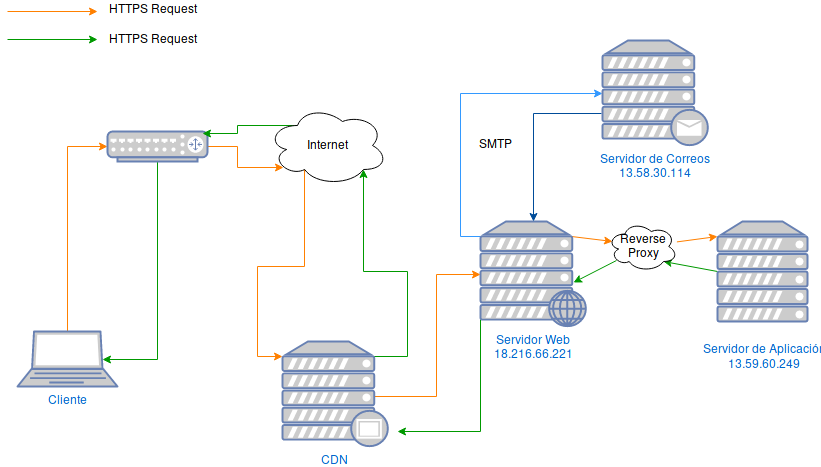
\includegraphics[width=0.8\linewidth]{net_diagram}
  \caption{Diagrama de red de los servidores web, de aplicación y de correo electrónico}
\end{figure}

\subsection{DNS}
El servicio de \textsf{DNS} que utilizamos es \textsf{Route 53} de Amazon, pues está integrado en la misma plataforma que los servidores y al ser diseñados para trabajar en conjunto, la integración fue mucho más fácil que con Cloudflare.
\begin{figure}[H]
  \centering
  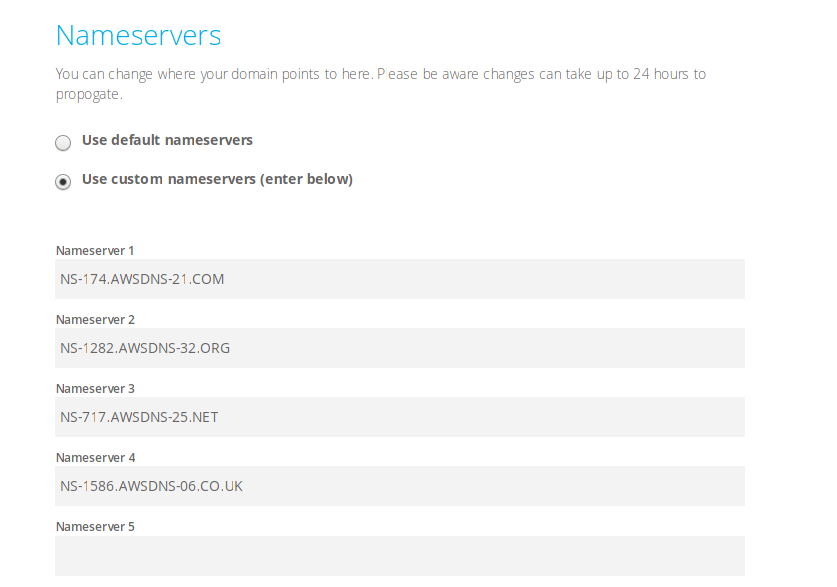
\includegraphics[width=0.8\linewidth]{nameservers}
  \caption{Nameservers de Amazon agregados en la configuración de freenom}
\end{figure}
\begin{figure}[H]
  \centering
  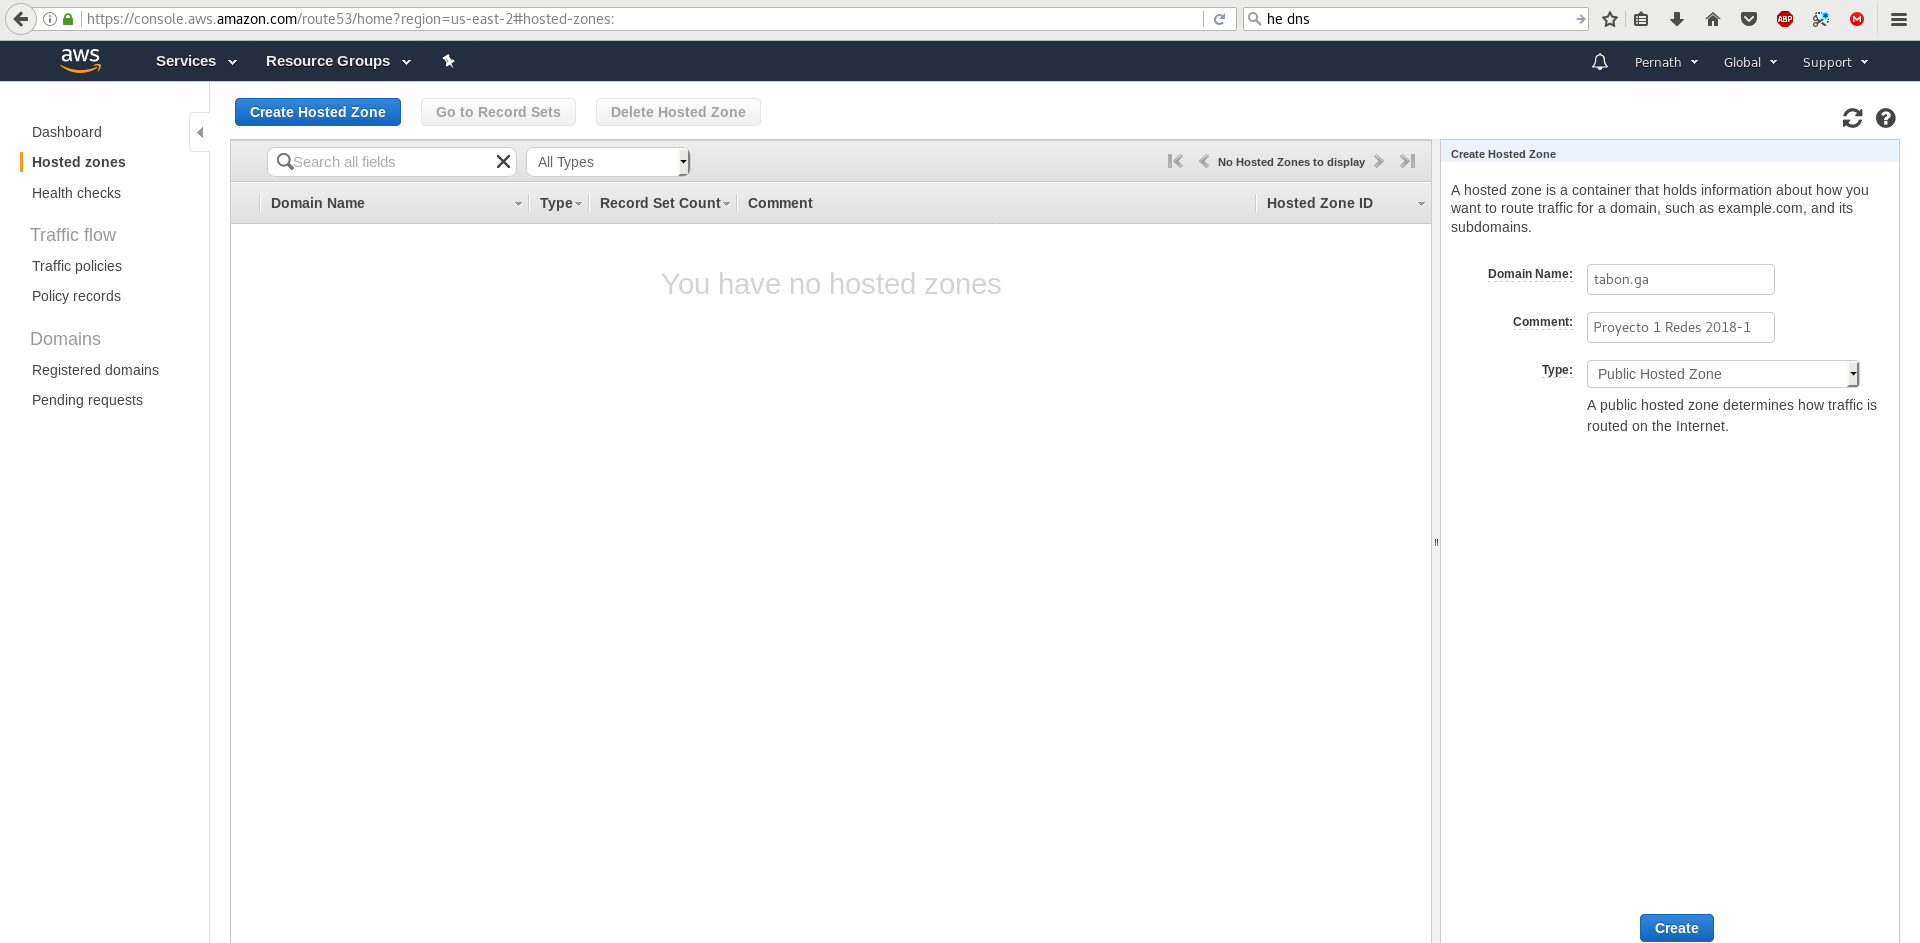
\includegraphics[width=0.8\linewidth]{DNS_management}
  \caption{Panel de control de Route 53 sin zonas creadas}
\end{figure}
\begin{figure}[H]
  \centering
  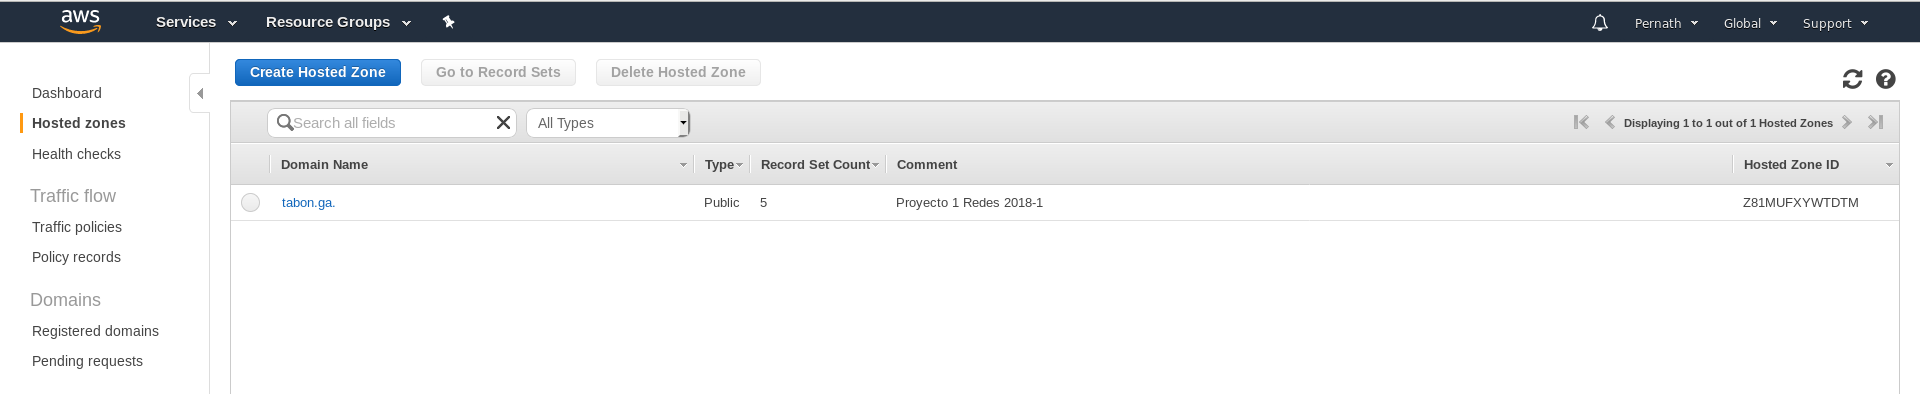
\includegraphics[width=0.8\linewidth]{HostedZones}
  \caption{zonas creadas}
\end{figure}
\begin{figure}[H]
  \centering
  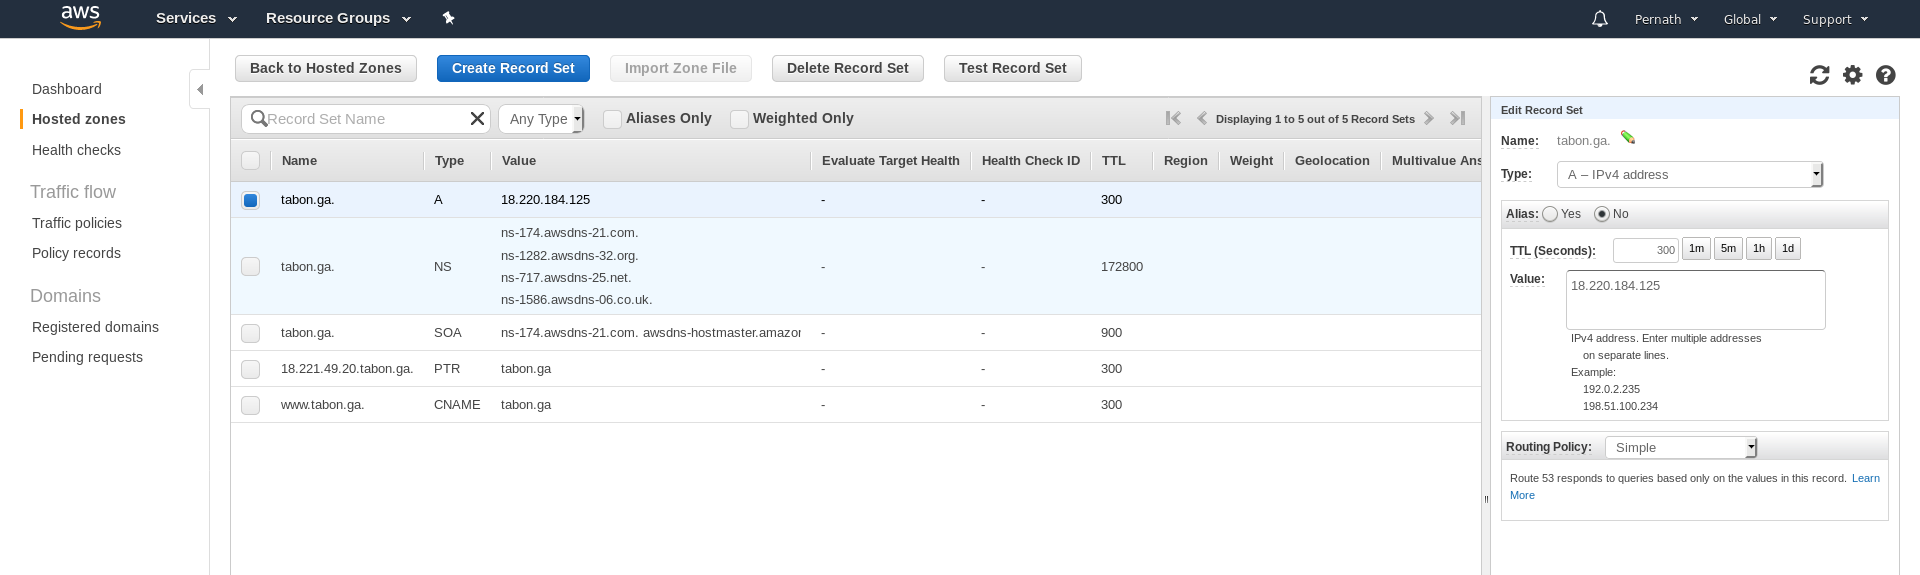
\includegraphics[width=0.8\linewidth]{A}
  \caption{Detalles del registro A para IPv4}
\end{figure}
\begin{figure}[H]
  \centering
  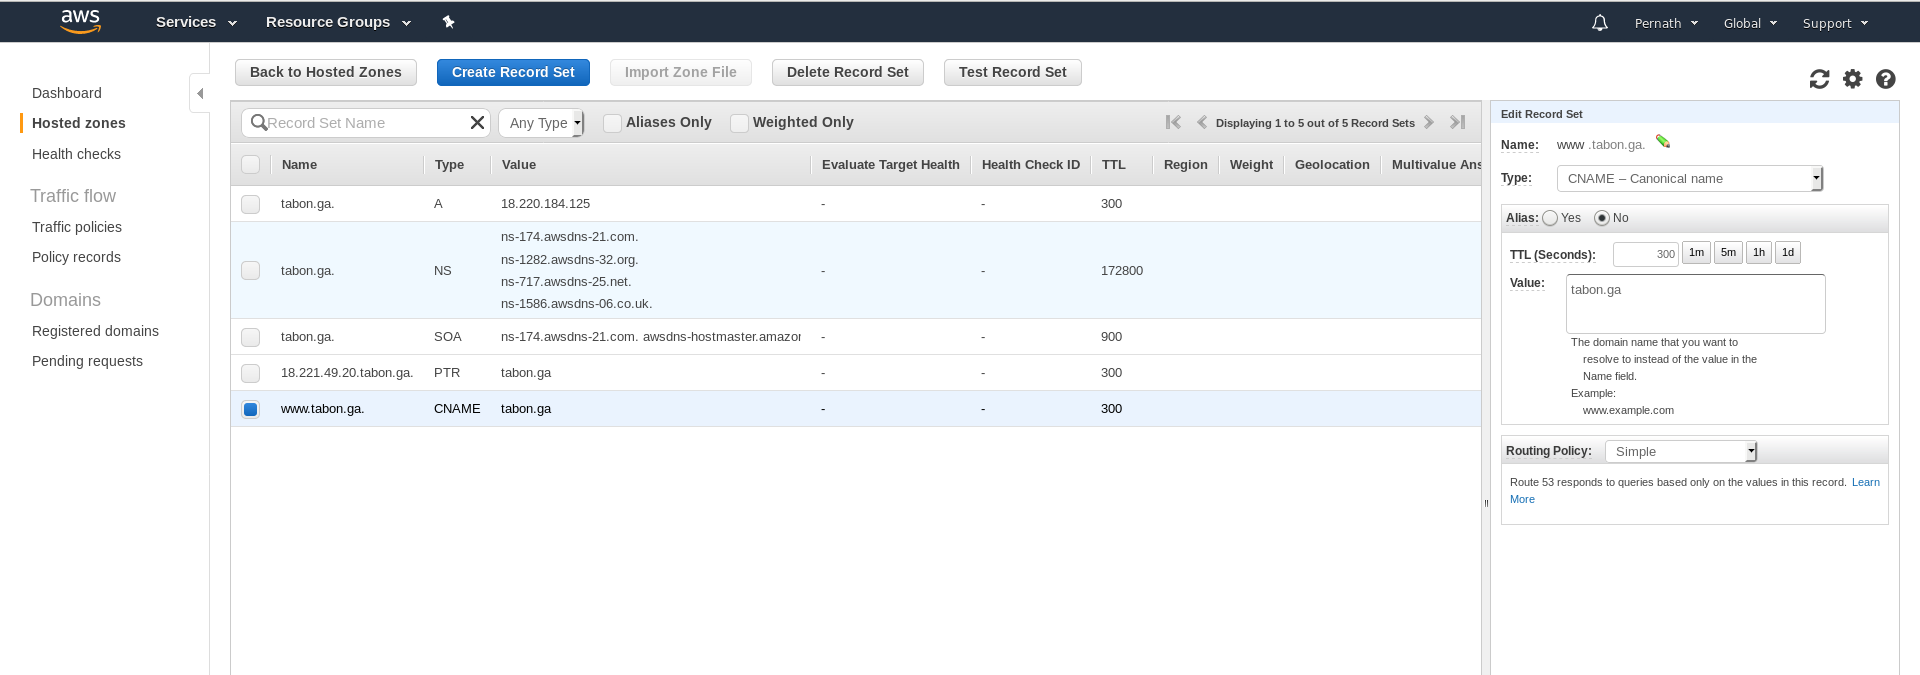
\includegraphics[width=0.8\linewidth]{CNAME}
  \caption{Detalles del registro CNAME para nombre canónico}
\end{figure}
\begin{figure}[H]
  \centering
  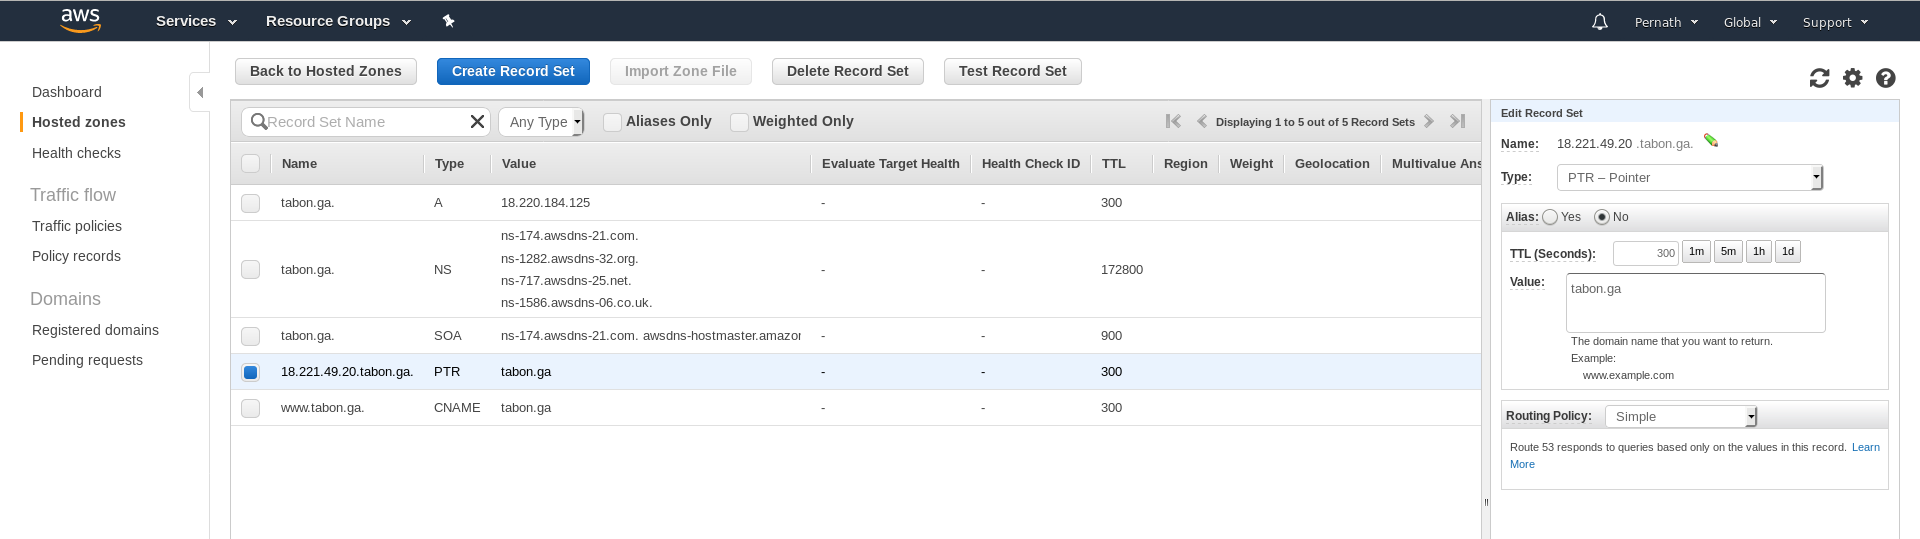
\includegraphics[width=0.8\linewidth]{PTR}
  \caption{Detalles del registro PTR}
  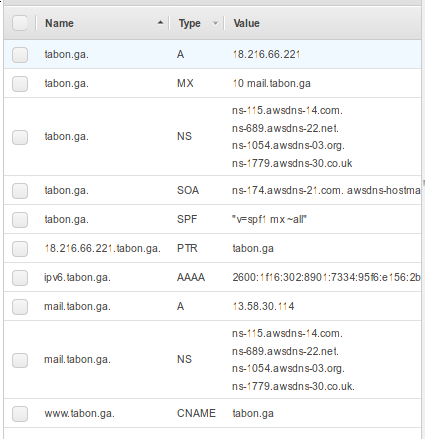
\includegraphics[scale=0.5]{record_set}
  \caption{Vista de todos los registros}
\end{figure}

\newpage

\subsection{Configuración de direcciones IPv4 e IPv6} 
Se usaron 3 instancias de la plataforma \textsf{EC2} de Amazon para los servidores de la aplicación, cada una con la distribución \textsf{Ubuntu 16.04} y con manejo a través de \textsf{ssh}. 
\begin{figure}[H]
  \centering
  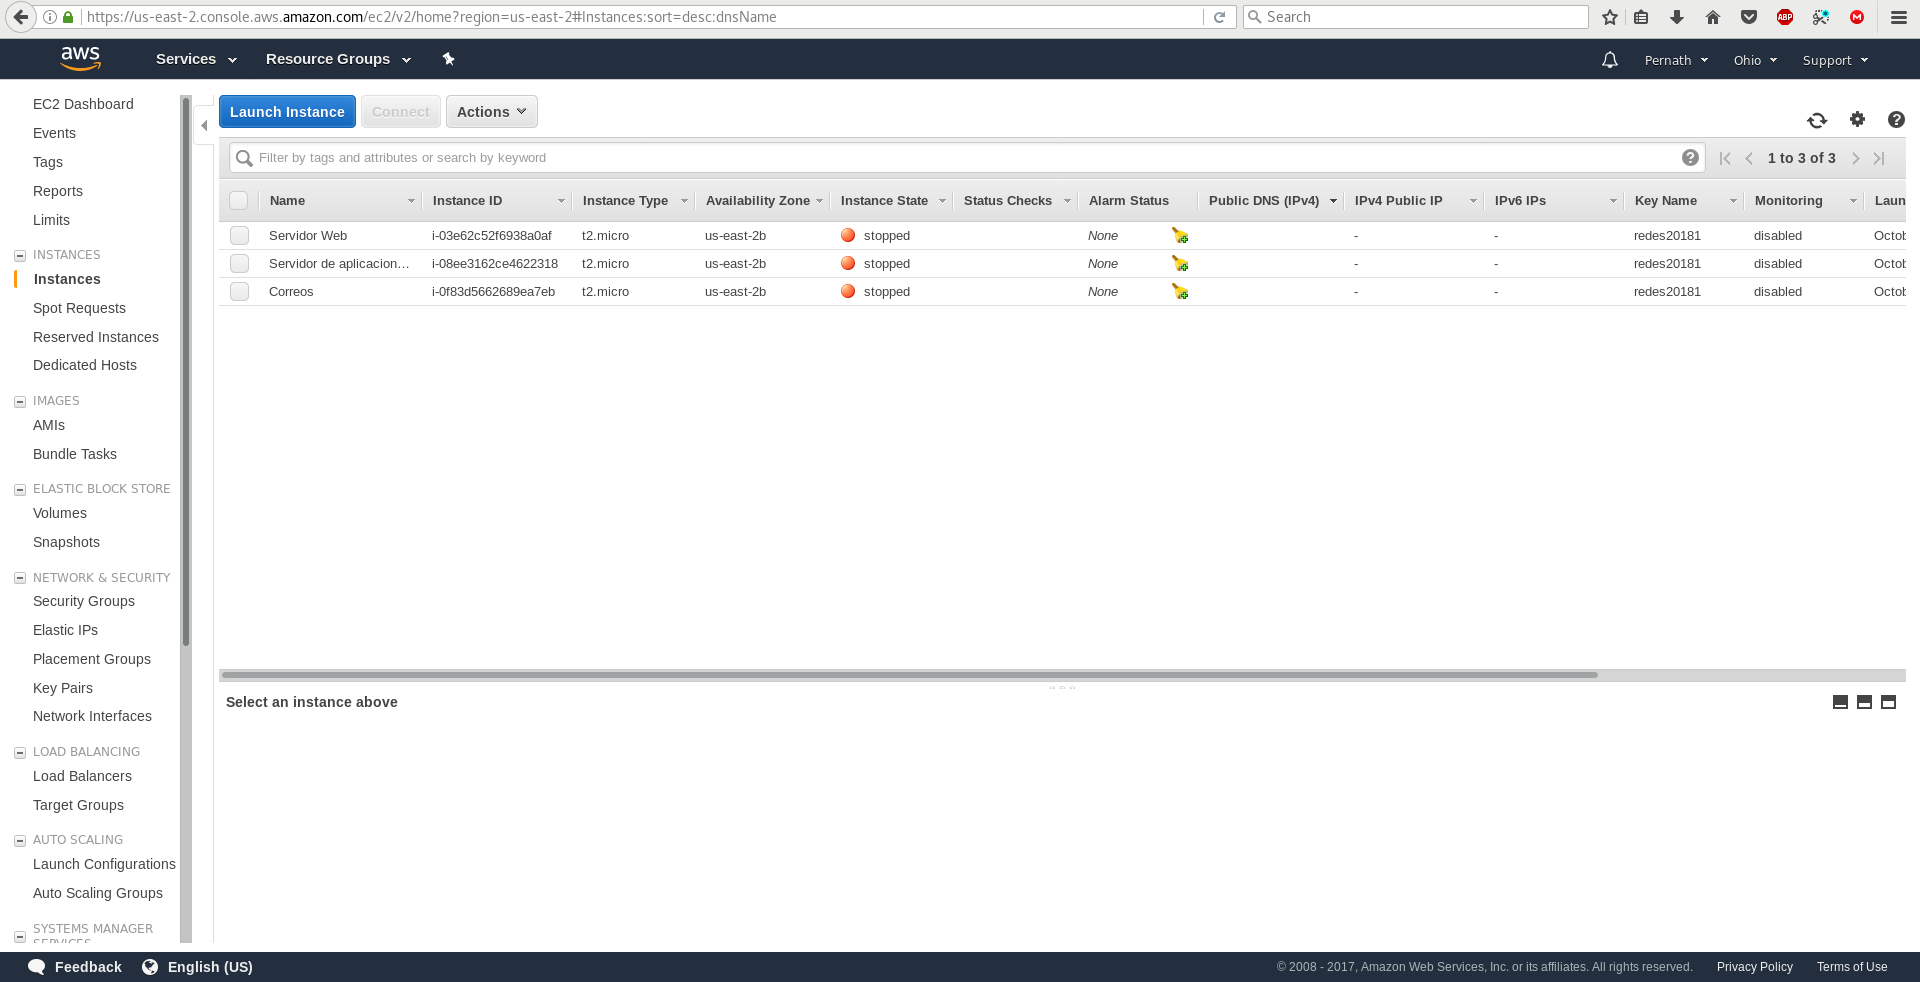
\includegraphics[width=\textwidth]{instances_dashboard}
  \caption{panel de control de las VPS}
\end{figure}
\begin{figure}[H]
  \centering
  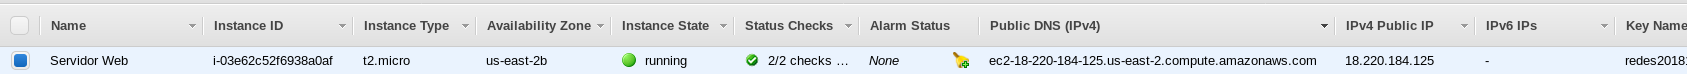
\includegraphics[width=\textwidth]{web_server}
  \caption{Servidor web en ejecución}
\end{figure}

\subsubsection{Configuración de IPv4 públicas}
Por defecto, \textsf{AWS} asigna direcciones IP públicas para las máquinas de manera dinámica. Es decir, cada vez que la instancia se inicializa después de haber sido detenida obtiene una IP pública diferente, lo que genera problemas al agregar servicios como DNS. Sin embargo, el mismo \textsf{Amazon EC2} proporciona una herramienta que nos permite obtener IPv4 estáticas para nuestras instancias y las llaman \textit{direcciones IP elásticas}.\\

Para asignar una dirección IP elástica debemos ingresar en la consola y \textsc{AWS} para \textsf{EC2} y en el panel de navegación de la izquierda seleccionar la opción \textbf{Elastic IPs}.\\
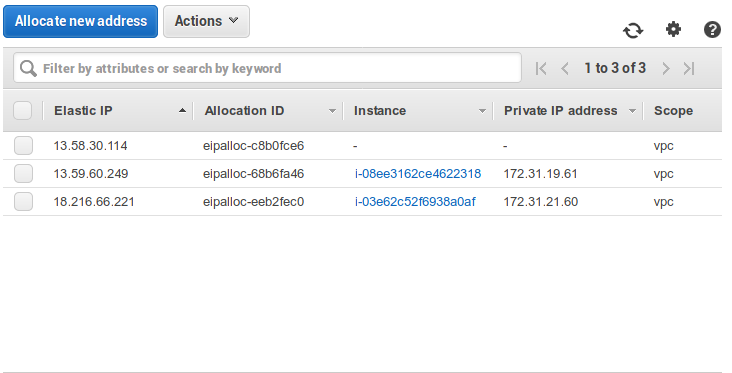
\includegraphics[width=\textwidth]{elastic_ip}
\\
Elegimos \textbf{Allocate new address} para obtener una nueva dirección elástica y luego confirmamos con \textbf{Allocate}
\begin{figure}[H]
  \centering
  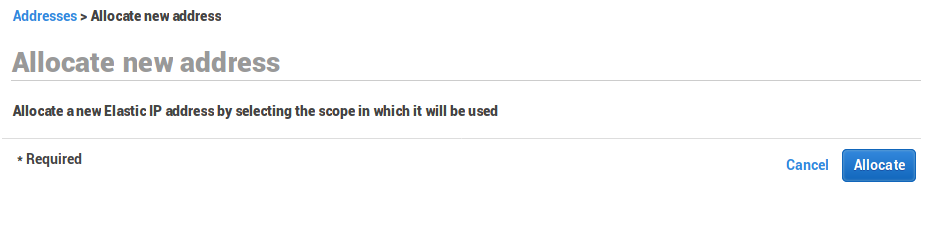
\includegraphics[width=\textwidth]{elastic_ip_allocate}
  \caption{Asignación de IP elástica}
\end{figure}

\begin{figure}[H]
  \centering
  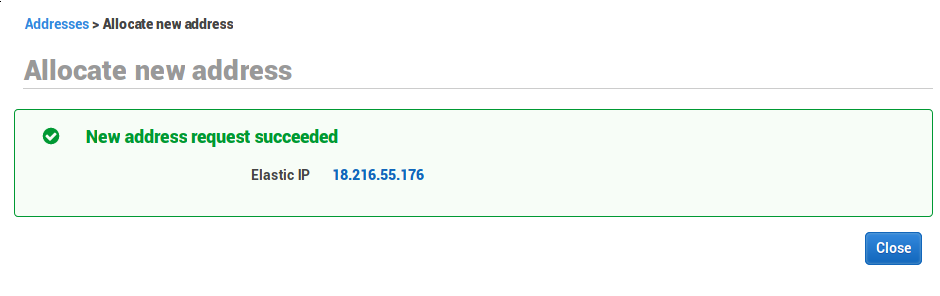
\includegraphics[width=\textwidth]{elastic_ip_success}
  \caption{Mensaje de éxito en la asignación de la dirección}
\end{figure}

Para asociar una dirección elástica a una instancia en ejecución nuevamente ingresamos en la opción \textbf{Elastic IPs} del panel de navegación de la consola de \textsf{EC2}. \\
%no ss
Elegimos la dirección que recien se nos asignó y en su menu \textbf{Action} elegimos la opción \textbf{Associate address}. \\
Luego seleccionamos la instancia a la que queramos asociar la IPv4 pública y damos click en \textbf{Associate}.

\subsubsection{Configuración de IPv6}
Para la asignación de IPv6 necesitamos crear una \textit{gateway} de solo salida a traves de una \textsf{VPC} (Virtual Private Cloud). Esta gateway les permite a las máquinas que estén en la VPC establecer conexiones por IPv6 a Internet, pero impide que se hagan conexiones por IPv6 con las instancias desde algún lugar en internet.
\\
\begin{figure}[H]
  \centering
  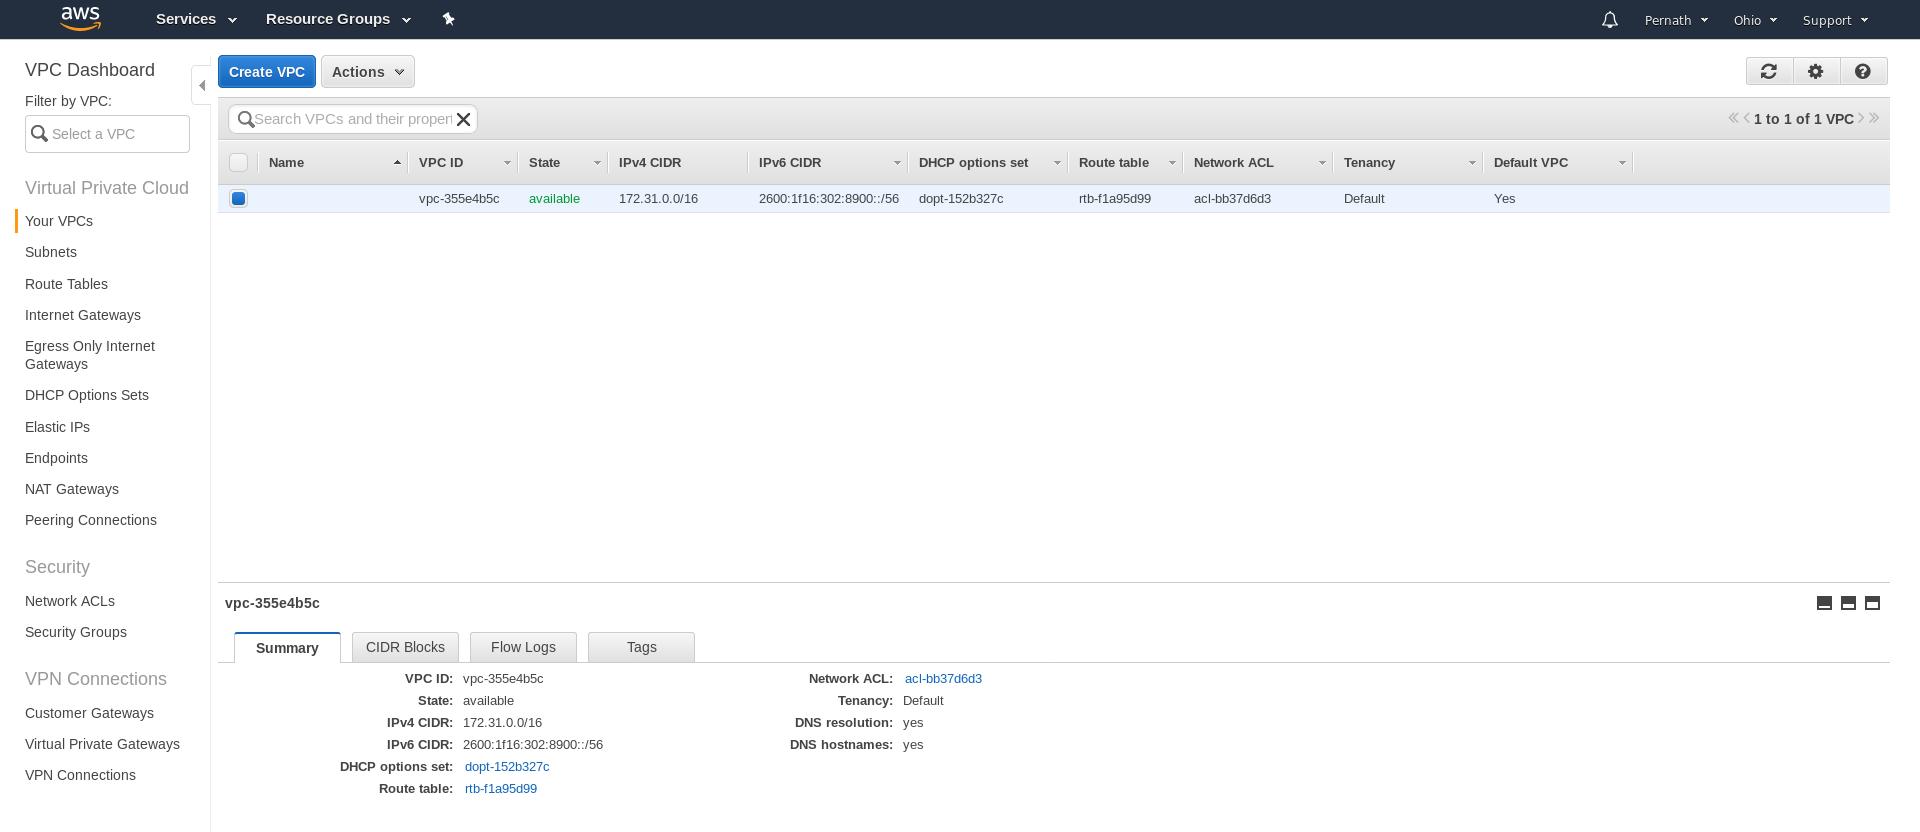
\includegraphics[width=0.8\linewidth]{vpc}
  \caption{Creación de una VPC para las instancias de EC2}
\end{figure}
\begin{figure}
  \centering
  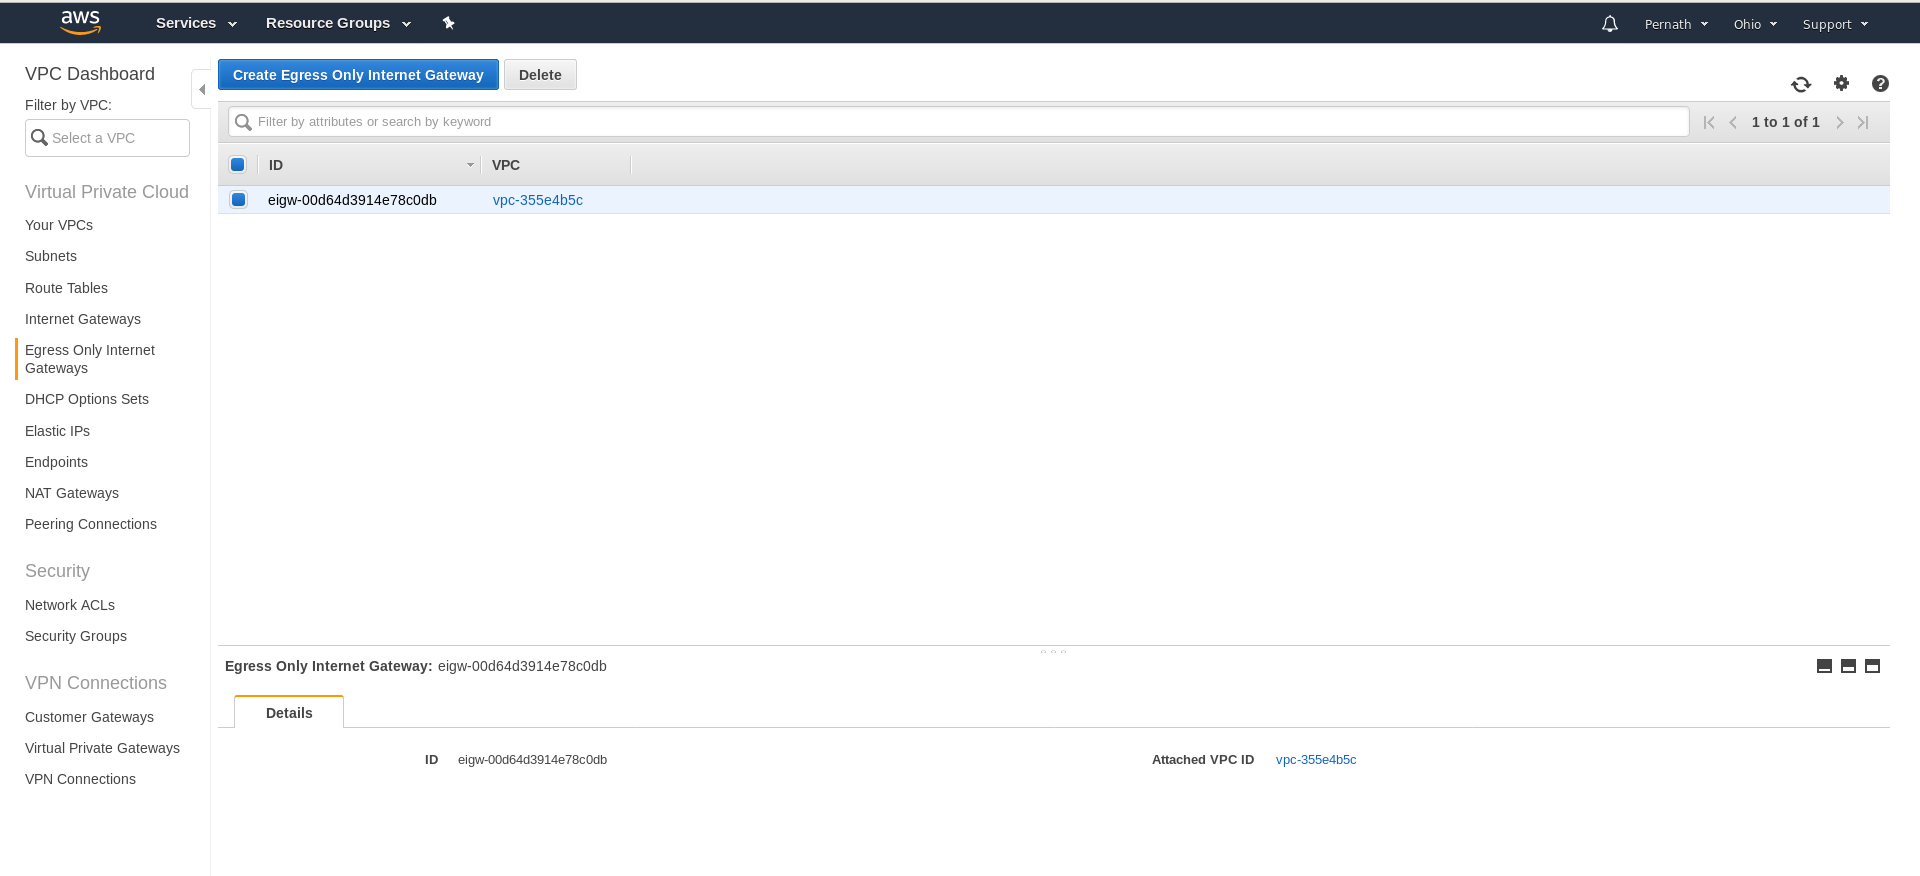
\includegraphics[width=0.8\linewidth]{vpc_egress_only}
  \caption{En el panel de VPC aparece la opción de crear una gateway de solo salida para la VPC que elijamos}
\end{figure}
\begin{figure}[H]
  \centering
  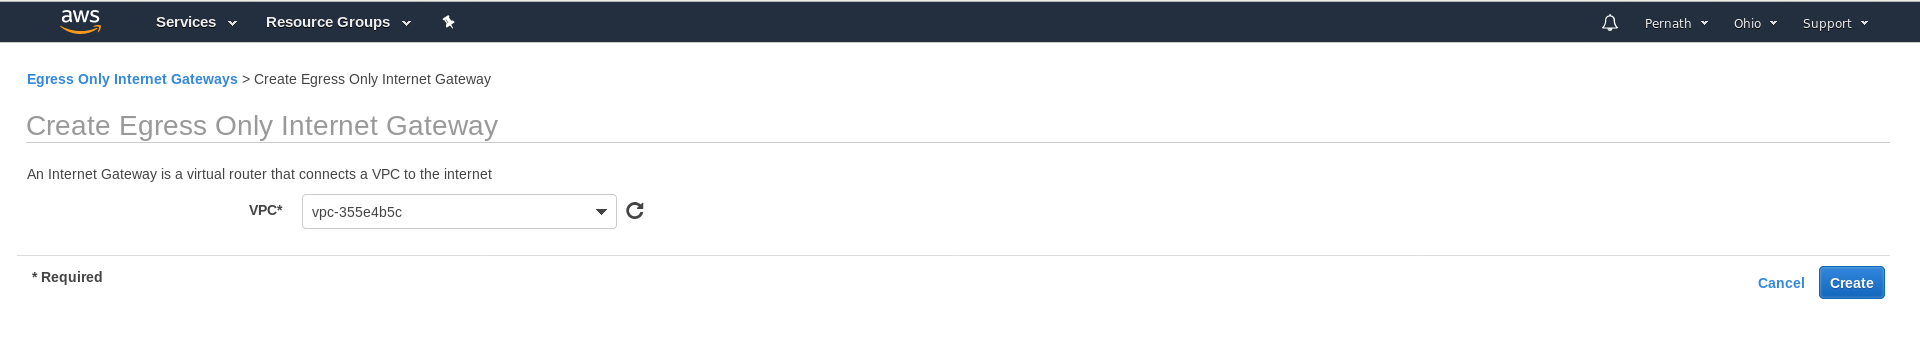
\includegraphics[width=0.8\linewidth]{egress_only_gateway}
  \caption{Creación de la gateway de solo salida para la VPC que contiene nuestras instancias de EC2}
\end{figure}
\begin{figure}[H]
  \centering
  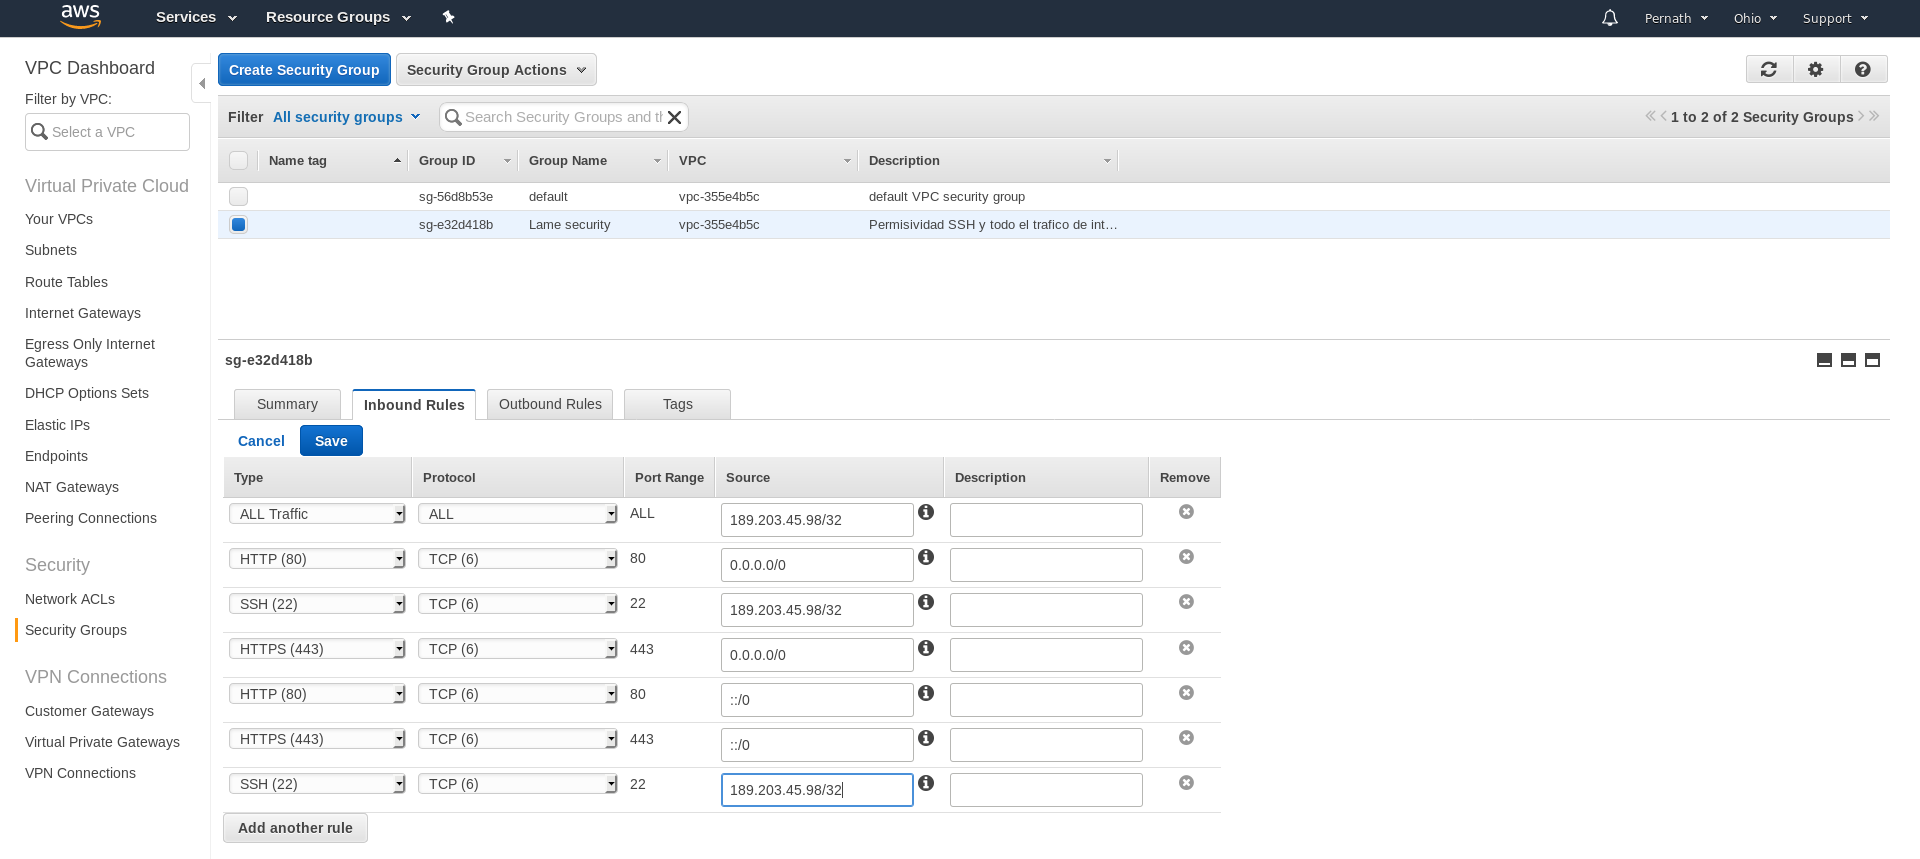
\includegraphics[width=0.7\textwidth]{edit_security_group}
  \caption{Editamos el grupo de seguridad (firewall) para que permita el tráfico  de salida de la VPC}
\end{figure}

\begin{figure}[H]
  \centering
  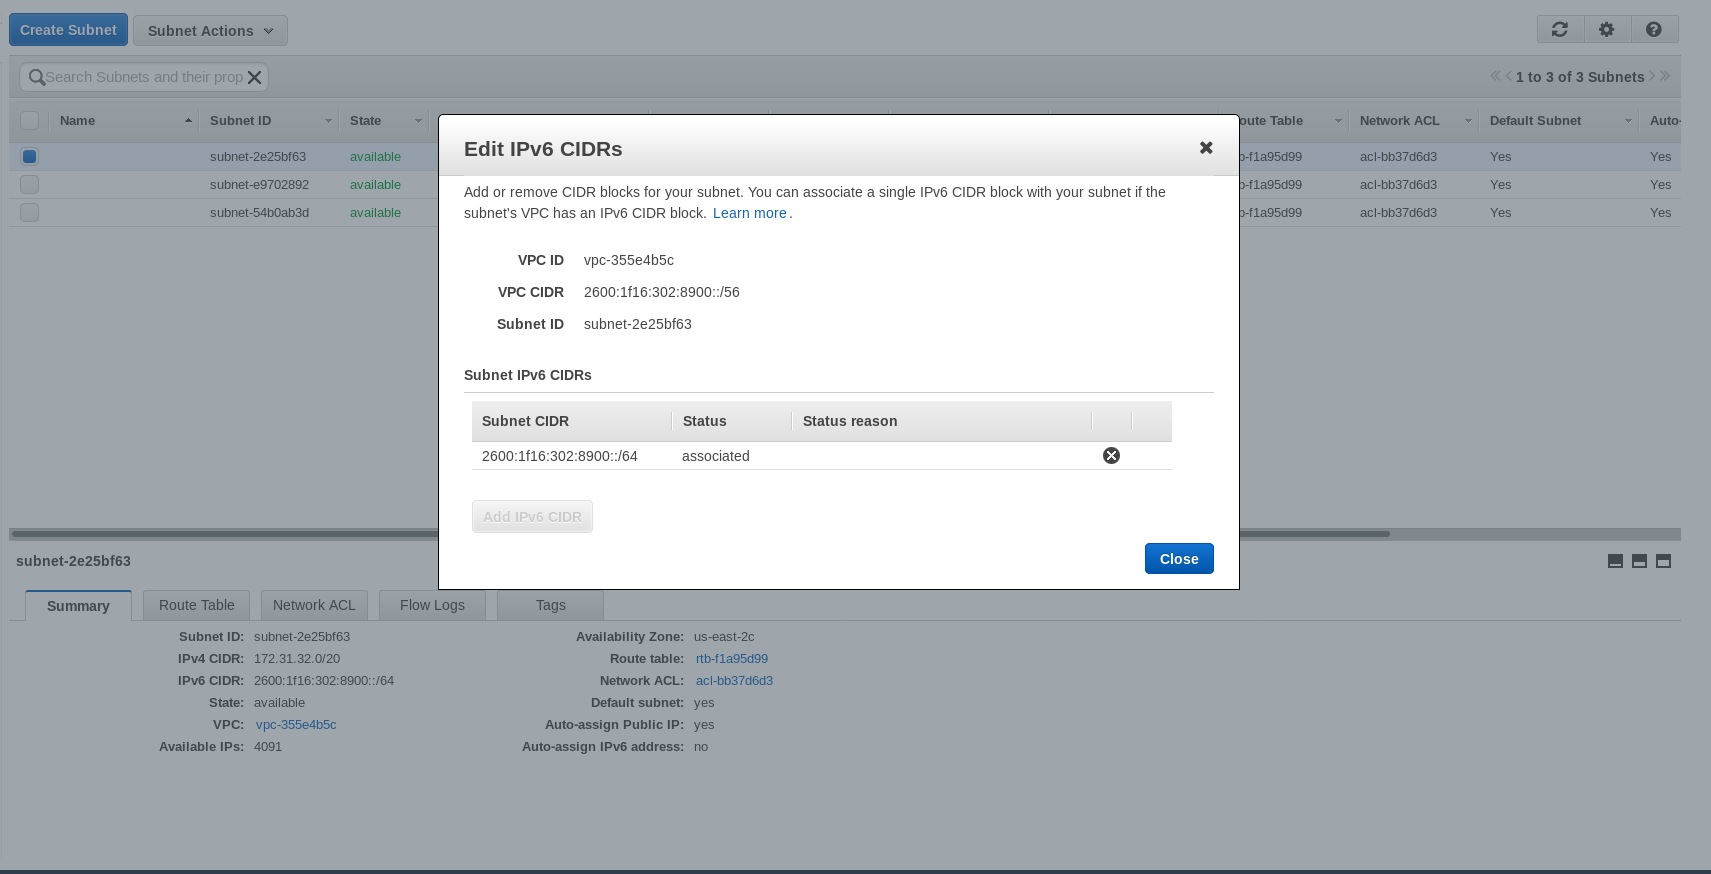
\includegraphics[width=0.7\textwidth]{ipv6_cidr}
  \caption{Creación del bloque CIDR para la generación de direcciones IPv6 públicas}
\end{figure}

\begin{figure}[H]
  \centering
  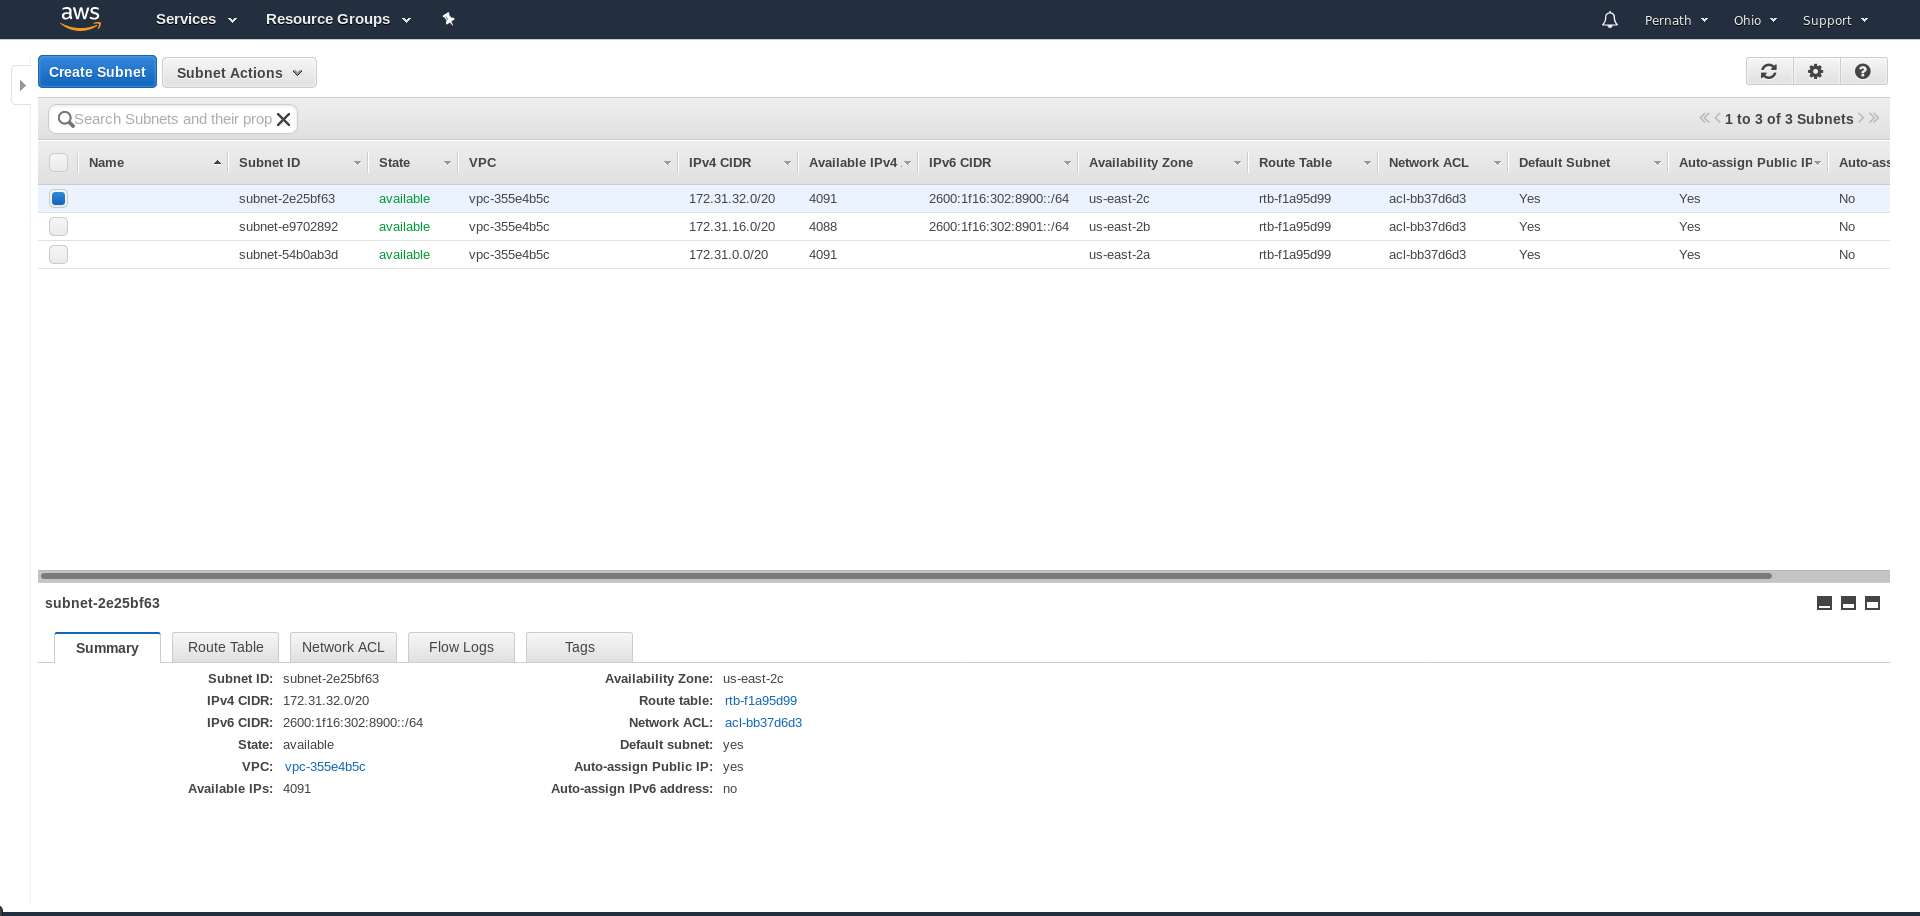
\includegraphics[width=0.7\textwidth]{subnets}
  \caption{Subredes para las instancias}
\end{figure}

\begin{figure}[H]
  \centering
  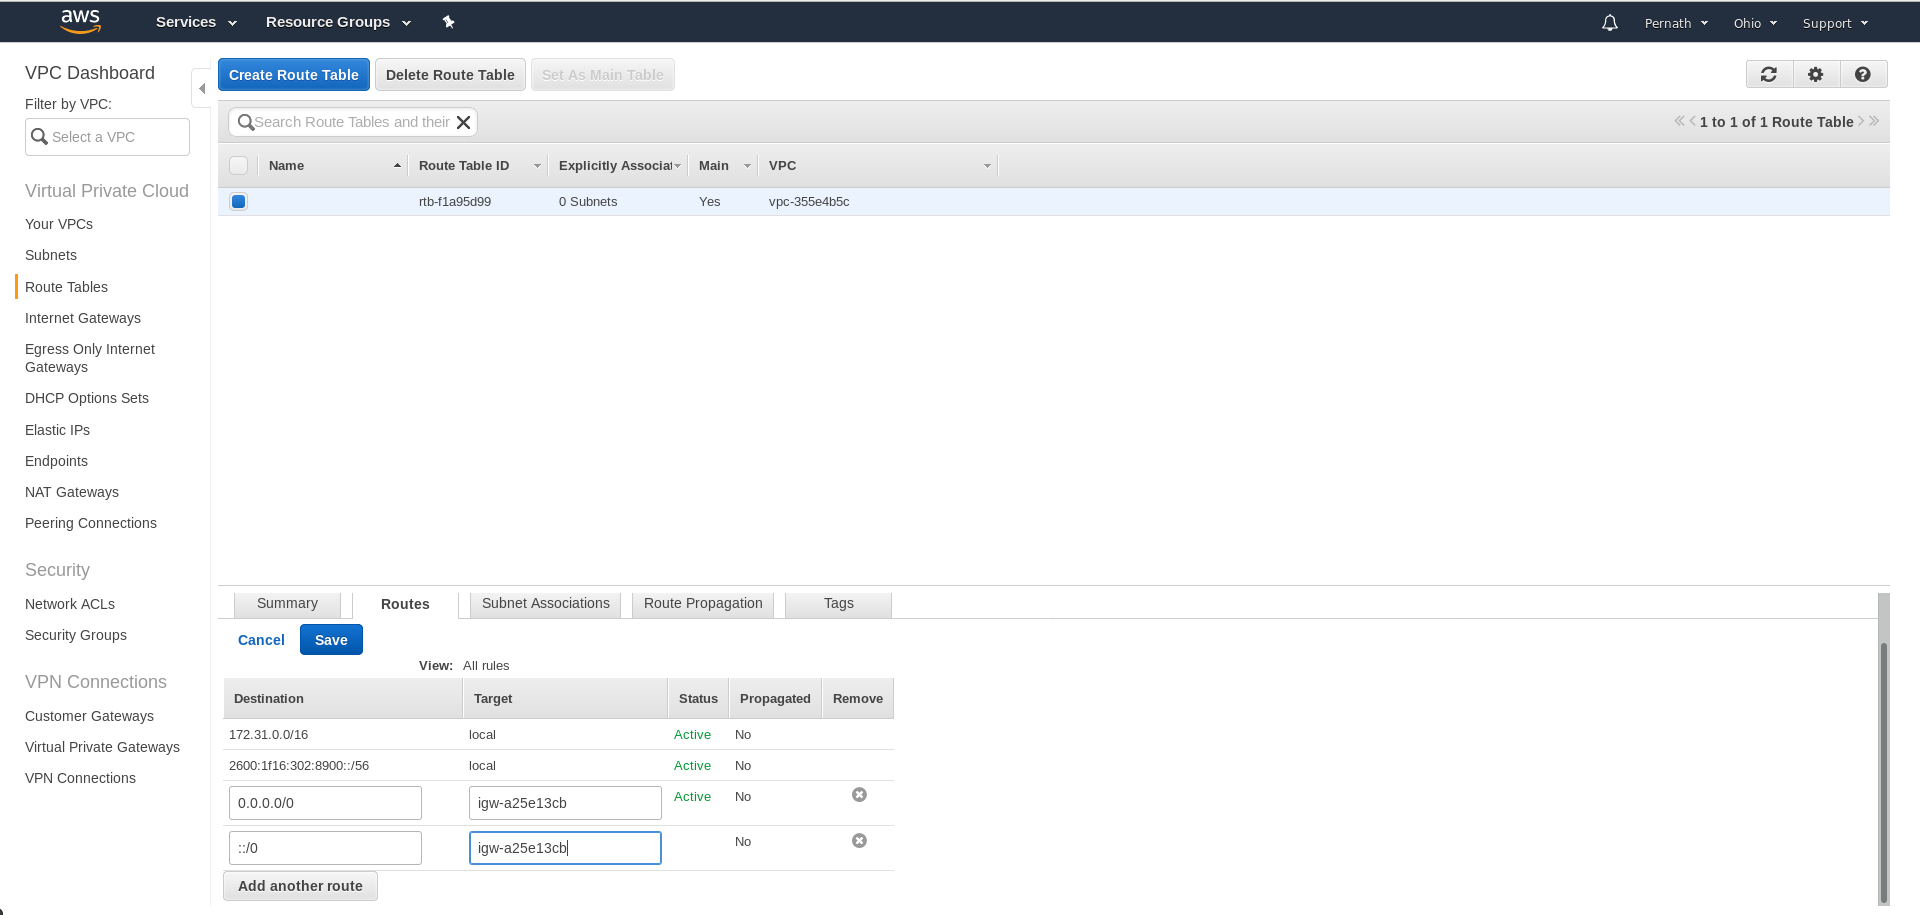
\includegraphics[width=0.7\textwidth]{public_subnet}
  \caption{Subred pública en la VPC para asignarles direcciones generadas por el bloque CIDR}
\end{figure}

\begin{figure}[H]
  \centering
  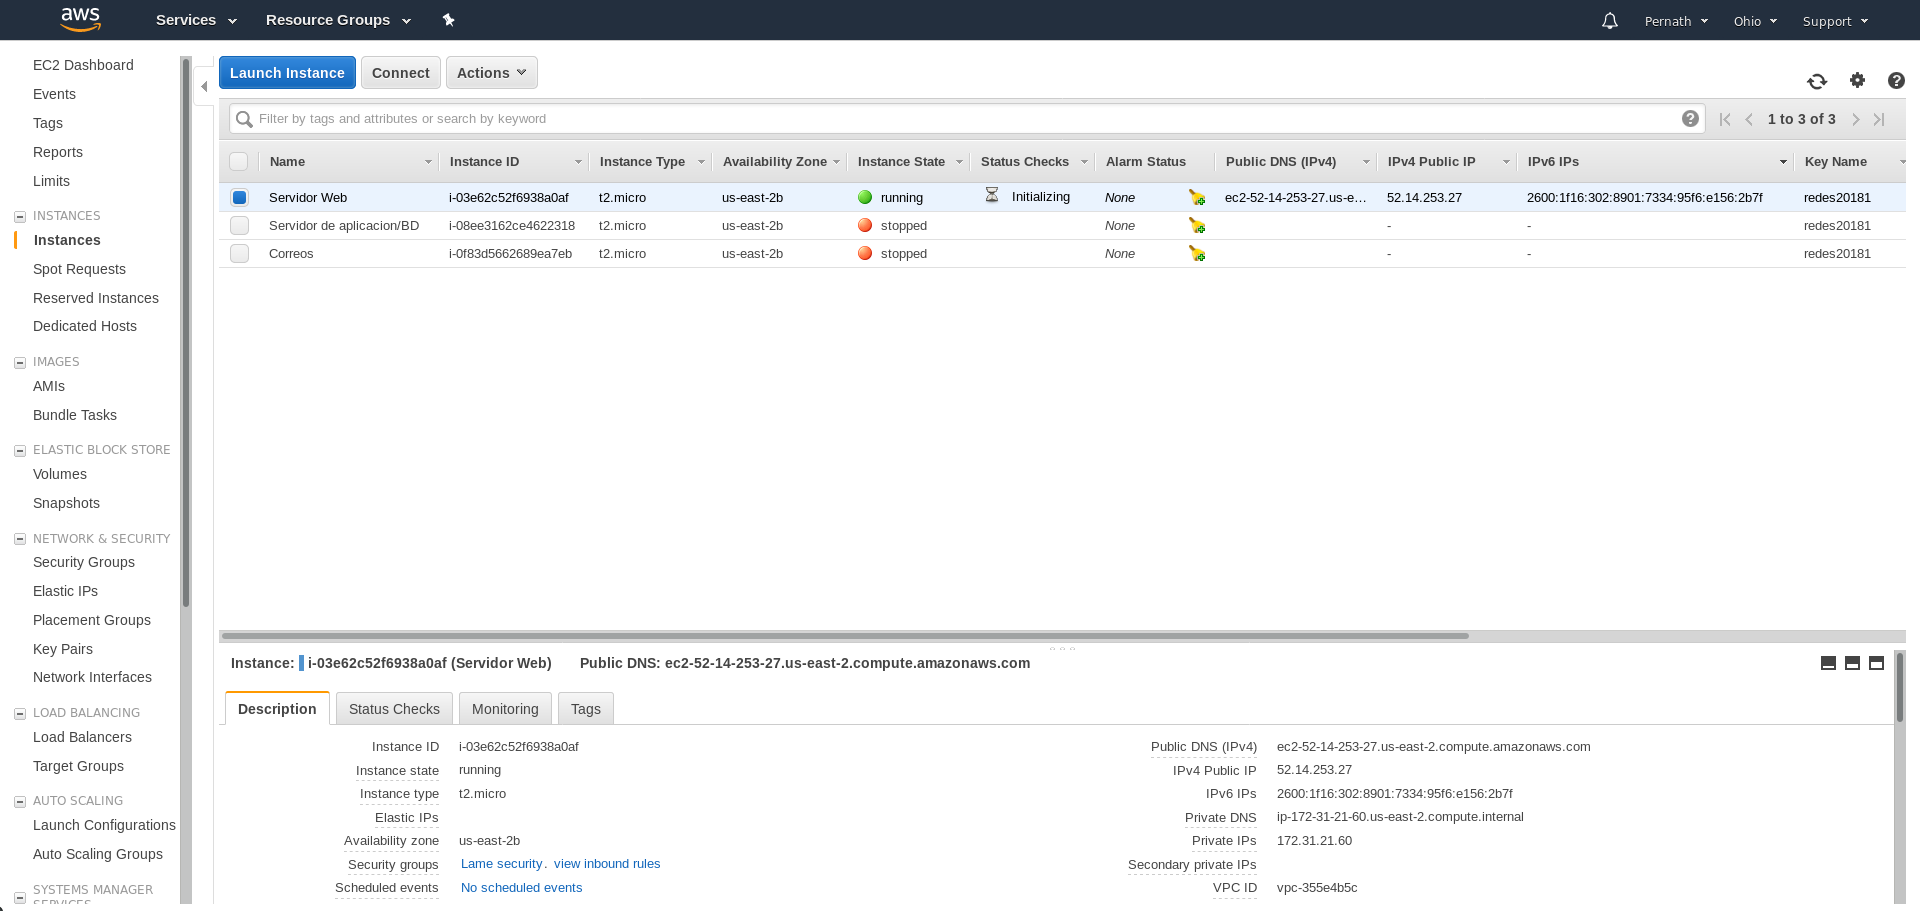
\includegraphics[width=0.7\textwidth]{ipv6_assignment}
  \caption{Asignación de direcciones IPv6 a los servidores}
\end{figure}

\section{Servidor de Aplicación}

\subsection{Diagrama de la base de datos}
Dada la simpleza de la aplicación, la base de datos solo cuenta con una tabla para los usuarios con sus respectivos atributos.\\
\begin{figure}[H]
  \centering
  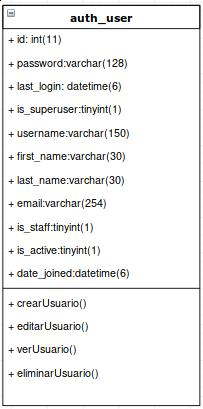
\includegraphics[scale=0.5]{db}
  \caption{Tabla de usuario}
\end{figure}

%\vspace{2cm} %it just works

\subsection{Objetivo de la aplicación}
La aplicación fue desarrollada con el fin de ilustrar las funciones básicas de una aplicación web con base de datos, es decir, \textit{crear, editar, ver y liminar} y que pueden asociarse a distintos métodos \textsf{HTTP} de la capa de aplicación como \textsf{PUT, POST, GET, PATCH o DELETE}. \\
A partir de esta pequeña aplicación \textit{CRUD} puede escalarse a proyectos más grandes y de mayor comp1lejidad gracias a la escalabilidad de \textbf{Django}, el framework usado.

\subsection{Uso de la aplicación}
Al ingresar al sitio, el usuario se encontrará con dos enlaces: uno para registrarse en la plataforma y otro para iniciar sesión en ésta.
\begin{figure}[H]
  \centering
  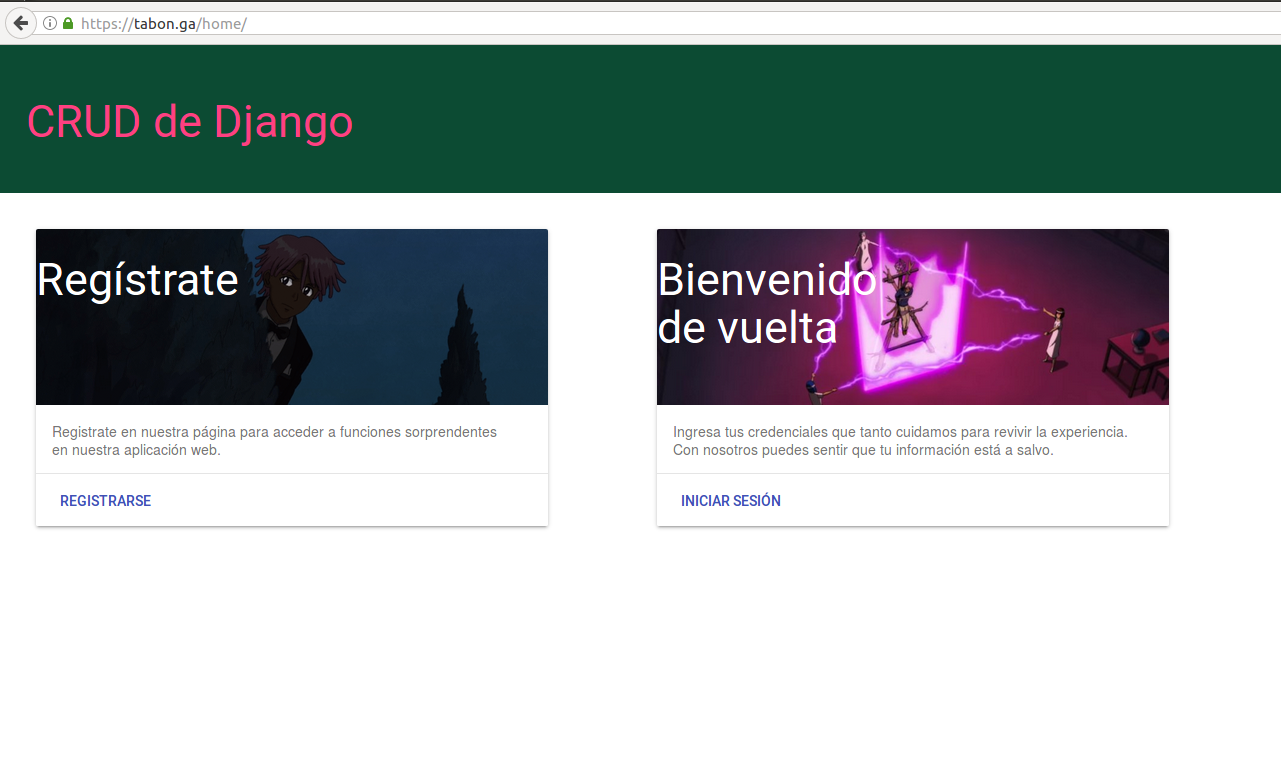
\includegraphics[width=\textwidth]{crud/app1}
  \caption{Página de inicio para usuarios sin sesión activa}
\end{figure}

Si no está registrado e ingresa en el enlace para registrarse, será redireccionado a un formulario para que llene sus datos y se de de alta en la aplicación.

\begin{figure}[H]
  \centering
  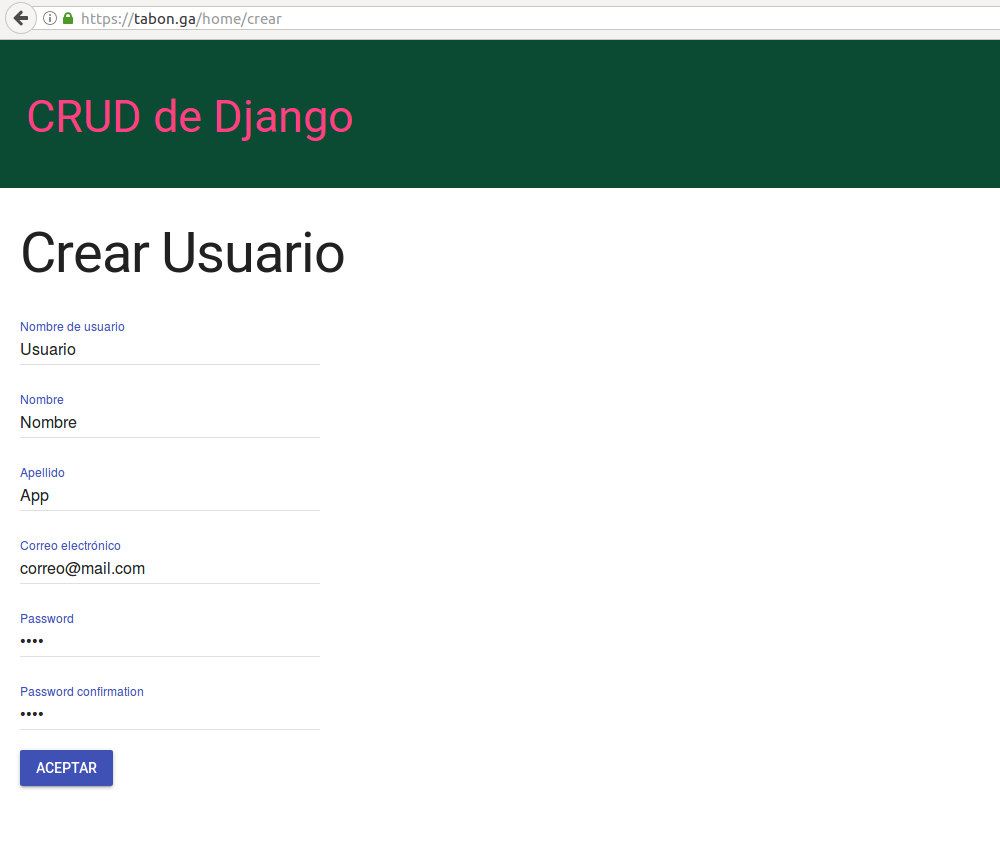
\includegraphics[width=\textwidth]{crud/app2}
  \caption{Formulario de registro para usuarios}
\end{figure}

Si ya está registrado, podrá ingresar a la aplicación siguiendo el enlace de \textit{Iniciar sesión} en la página de inicio y en el formulario escribir el nombre de usuario y la contraseña con los que se registró.
\begin{figure}[H]
  \centering
  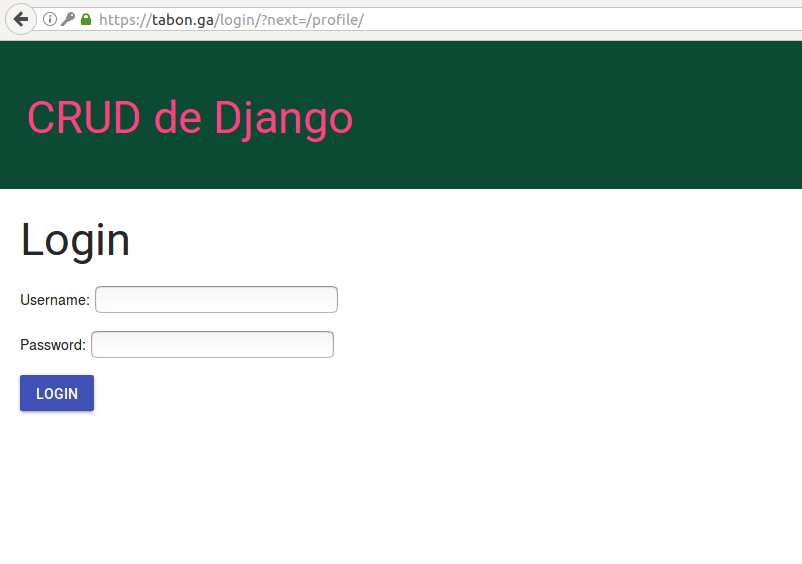
\includegraphics[width=\textwidth]{crud/app3}
  \caption{Formulario de inicio de sesión}
\end{figure}


Una vez dentro de la aplicación, el usuario verá una lista de los usuarios registrados y tendrá las opciones de ver información más detallada sobre algún usuario o sí mismo, actualizar sus datos o eliminar su cuenta si así lo desea.\\
\begin{figure}[H]
  \centering
  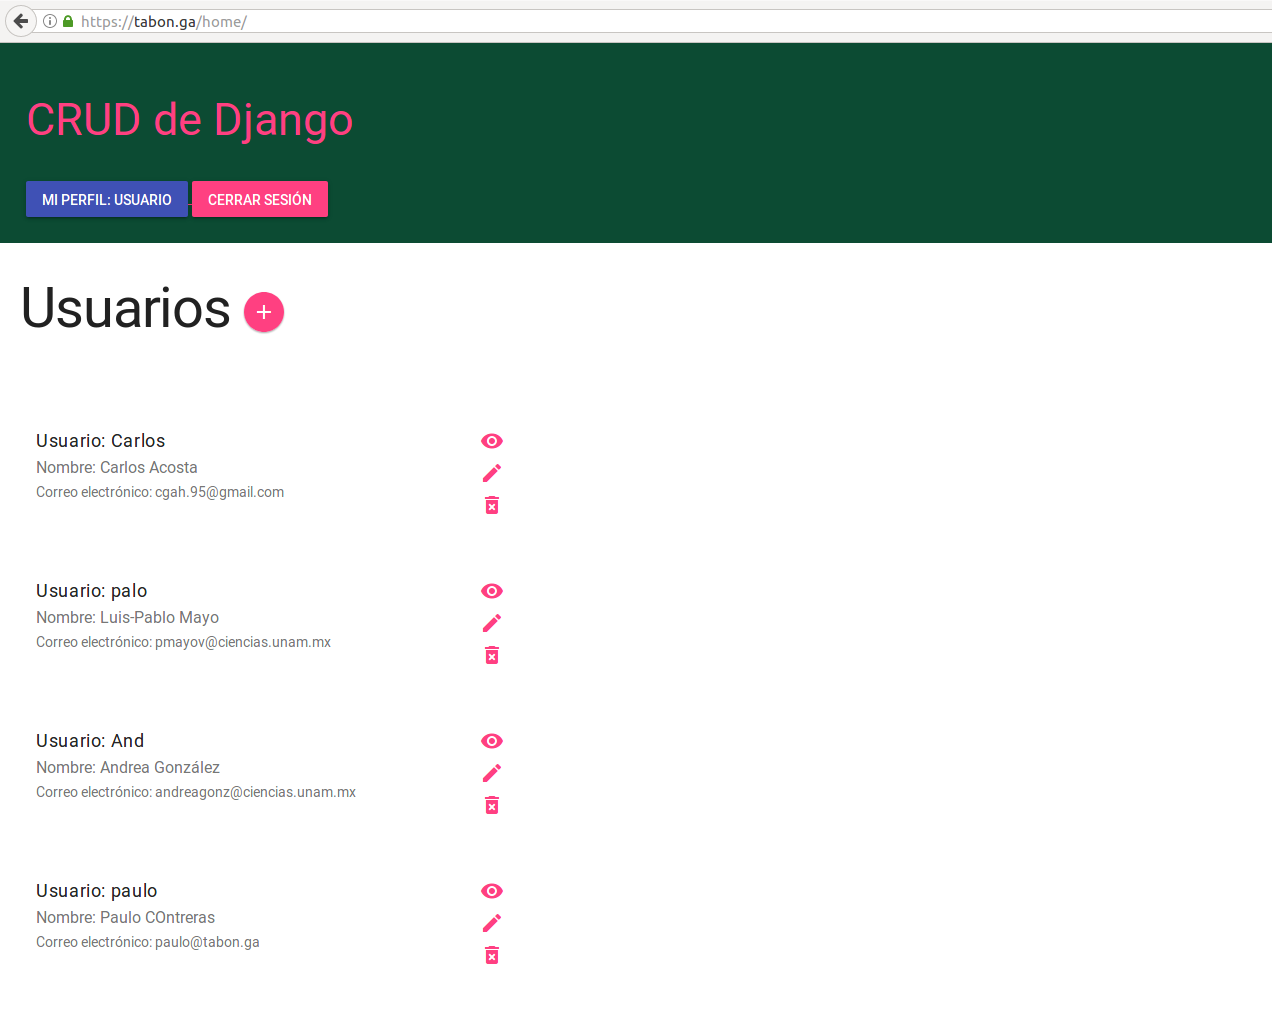
\includegraphics[width=\textwidth]{crud/app5}
  \caption{Página de inicio para usuarios con sesión activa}
\end{figure}

Si elige ver información más detallada sobre un usuario, el enlace lo llevará al perfil del usuario. \\
\begin{figure}[H]
  \centering
  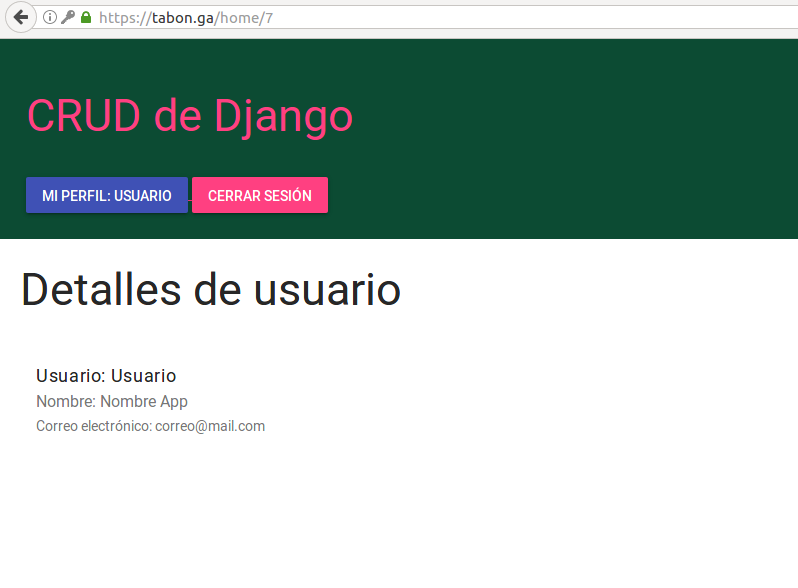
\includegraphics[width=\textwidth]{crud/app4}
  \caption{Perfil de usuario}
\end{figure}

Para actualizar sus datos, será redirigido a un formulario similar al de registro.\\
\begin{figure}[H]
  \centering
  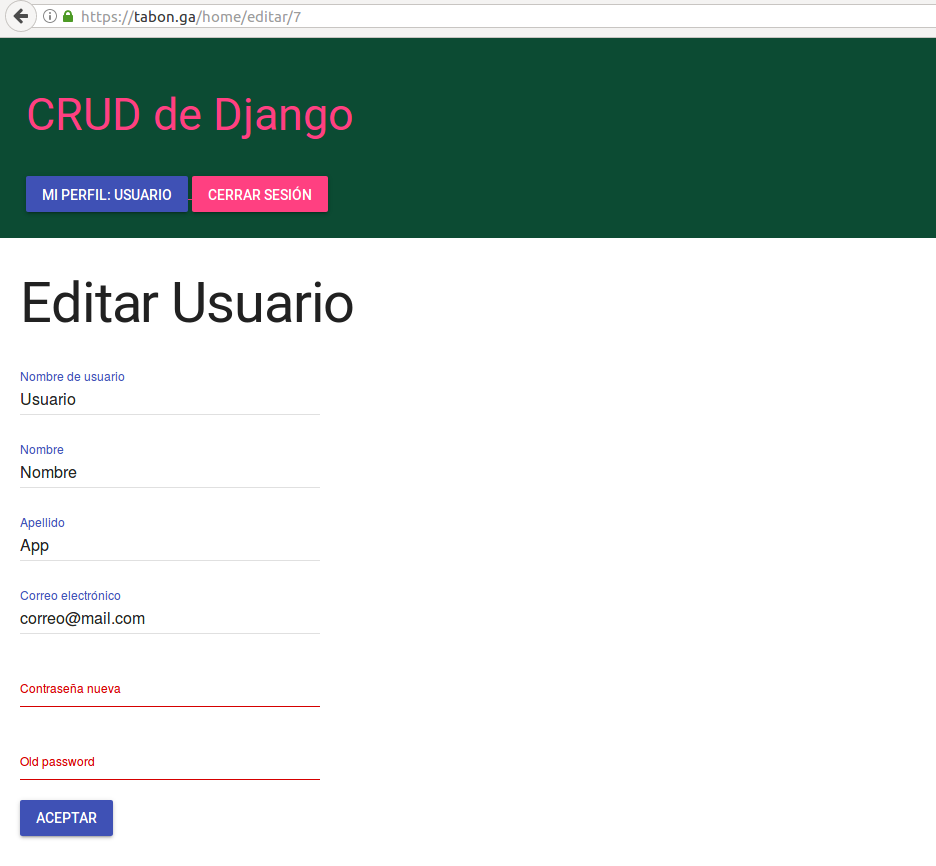
\includegraphics[width=\textwidth]{crud/app6}
  \caption{Formulario de actualización de datos}
\end{figure}

Si quiere eliminar su cuenta se le enviará un mensaje para que confirme su acción. \\
\begin{figure}[H]
  \centering
  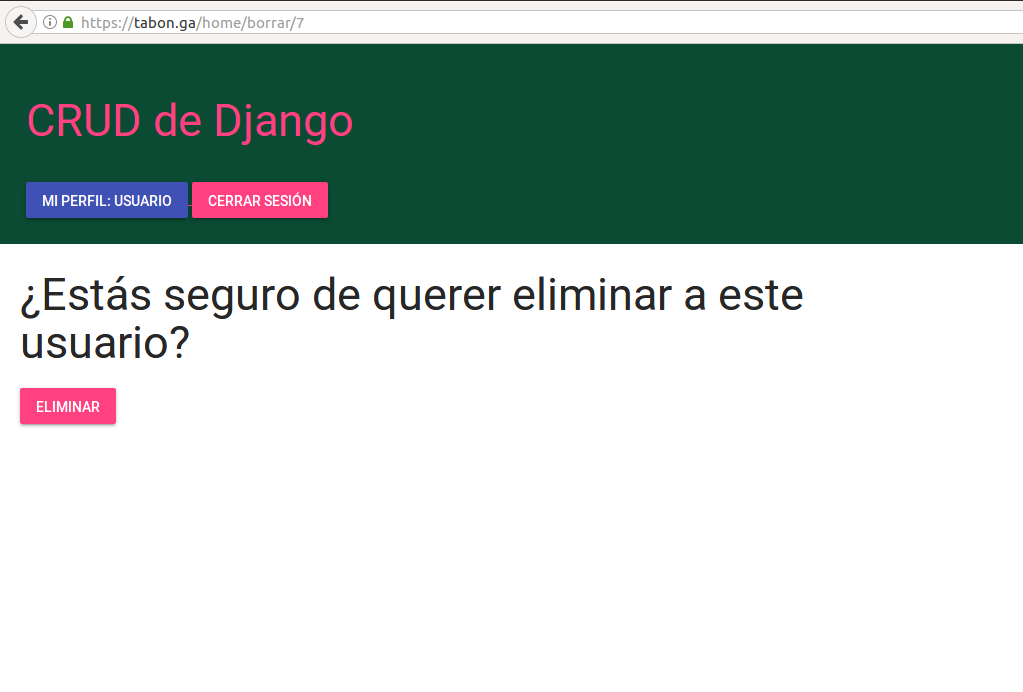
\includegraphics[width=\textwidth]{crud/app7}
  \caption{Mensaje de confirmación de eliminación de un usuario}
\end{figure}

\subsection{Gunicorn}

Para poder comunicar la aplicación con el servidor web instalamos \textsf{gunicorn}, que es un servidor web ligero que utiliza la interfaz WSGI para poder comunicarse con \textsf{python}.
\begin{verbatim}
    $ sudo apt-get install python3-pip
    $ sudo pip3 install gunicorn
\end{verbatim}

Creamos el archivo \texttt{/etc/systemd/system/gunicorn.service} para que \textsf{gunicorn} se ejecute con \textsf{systemd}.

\begin{verbatim}
[Unit]
Description=gunicorn daemon
After=network.target

[Service]
User=ubuntu
Group=www-data
WorkingDirectory=/home/ubuntu/djangocrud
ExecStart=/home/ubuntu/.local/bin/gunicorn --timeout 60 \
    --bind ec2-13-59-60-249.us-east-2.compute.amazonaws.com:8000 \
    djangocrud.wsgi:application

[Install]
WantedBy=multi-user.target
\end{verbatim}

Así, para ejecutar el demonio de \textsf{gunicorn} basta utilizar el comando
\begin{verbatim}
    $ systemctl start gunicorn
\end{verbatim}

\subsection{Reglas de firewall}

Definimos las siguientes reglas para el \textsf{firewall} que provee \textsf{Amazon}, de manera que se restringe la comunicación únicamente con el servidor web y a través de \textsf{SSH} por el puerto 2200.

\begin{figure}[H]
  \centering
  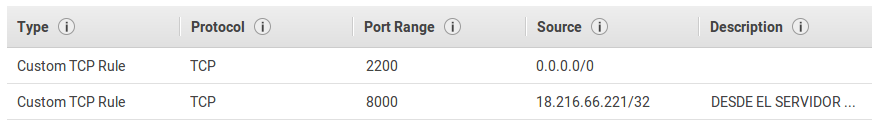
\includegraphics[width=\textwidth]{appsec}
  \caption{Reglas de \textsf{firewall} para el servidor de aplicación}
\end{figure}

\section{Servidor Web}

En el servidor web instalamos \textsf{apache2} con \texttt{sudo apt-get install apache2}, de modo que funcione como servidor de proxy inverso y mande las peticiones que reciba al servidor de aplicación y a su vez reciba respuestas de éste para mandárselas al cliente. \\

\subsection{Configuración de Apache}
Para la configuración de \textsf{apache2} modificamos los siguientes archivos como se muestra: \\

\texttt{/etc/apache2/sites-available/000-default.conf}

\begin{verbatim}
<VirtualHost *:80>
    ProxyPreserveHost On

    # Redirección a HTTPS
    RewriteEngine On
    RewriteCond %{HTTPS} !=on
    RewriteRule ^/?(.*) https://%{SERVER_NAME}/$1 [R,L]
    ServerName tabon.ga
</VirtualHost>
\end{verbatim}

\texttt{/etc/apache2/sites-available/default-ssl.conf}

\begin{verbatim}
<IfModule mod_ssl.c>
    <VirtualHost _default_:443>
        ServerAdmin webmaster@localhost
        DocumentRoot /var/www/html
        ErrorLog ${APACHE_LOG_DIR}/error.log
        CustomLog ${APACHE_LOG_DIR}/access.log combined
        SSLEngine on
        ServerName tabon.ga

        # Certificados de letsencrypt
        Include /etc/letsencrypt/options-ssl-apache.conf
        Include /etc/letsencrypt/options-ssl-apache.conf
        ServerAlias www.tabon.ga
        Include /etc/letsencrypt/options-ssl-apache.conf
        SSLCertificateFile    /etc/letsencrypt/live/tabon.ga/cert.pem
        SSLCertificateKeyFile    /etc/letsencrypt/live/tabon.ga/privkey.pem
        SSLCertificateChainFile    /etc/letsencrypt/live/tabon.ga/chain.pem
        <FilesMatch "\.(cgi|shtml|phtml|php)$">
            SSLOptions +StdEnvVars
        </FilesMatch>
        <Directory /usr/lib/cgi-bin>
            SSLOptions +StdEnvVars
        </Directory>

        # HSTS
        Header always set Strict-Transport-Security: \
            "max-age=31536000; includeSubDomains"
        RequestHeader set X-Forwarded-Proto 'https' env=HTTPS        
        Timeout 10000

        # Configuraciones del proxy inverso
        ProxyTimeout 10000
        ProxyBadHeader Ignore
        # Mandamos las peticiones del cliente al servidor de aplicación
        ProxyPass / http://13.59.60.249:8000/
        ProxyPassReverse / http://13.59.60.249:8000/
    </VirtualHost>
</IfModule>
\end{verbatim}

\texttt{/etc/apache2/conf-available/security.conf}

\begin{verbatim}
# Se deshabilita la firma de Apache para que no se muestre
# el nombre y version del sistema operativo
ServerTokens Prod
ServerSignature Off
TraceEnable Off
Header set X-Content-Type-Options: "nosniff"
\end{verbatim}

Habilitamos los siguientes módulos para hacer funcionar el proxy inverso y \textsf{SSL}.

\begin{verbatim}
    $ sudo a2enmod proxy_http
    $ sudo a2enmod proxy_ajp
    $ sudo a2enmod rewrite
    $ sudo a2enmod deflate
    $ sudo a2enmod headers
    $ sudo a2enmod proxy_balancer
    $ sudo a2enmod proxy_connect
    $ sudo a2enmod proxy_html
    $ sudo a2enmod lbmethod_byrequests
    $ sudo a2enmod ssl
\end{verbatim}

Finalmente, para habilitar \textsf{apache2} utilizamos
\begin{verbatim}
    $ sudo systemctl start apache2
\end{verbatim}

\subsection{Reglas de firewall}
\begin{figure}[H]
  \centering
  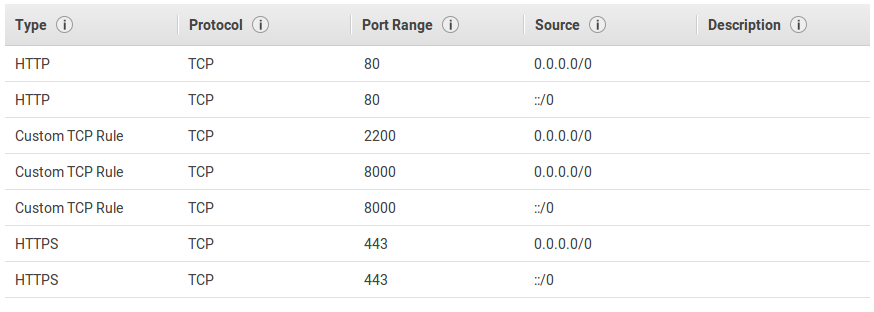
\includegraphics[width=\textwidth]{lamesec}
  \caption{Reglas de \textsf{firewall} para el servidor web}
\end{figure}


\section{\textit{Hardening}}
\subsection{Fail2ban}
Como los servidores tienen \textsf{Ubuntu} como sistema operativo, los archivos para la instalación de \textsf{fail2ban} están en los repositorios oficiales de la distribución, por lo que solo hizo falta ejecutar las instrucciones
\begin{verbatim}
# apt-get update
# apt-get install fail2ban
\end{verbatim}
Después de haber instalado \textsf{fail2ban} en el servidor, por recomendación de los desarrolladores, creamos un archivo \texttt{jail.local} como copia del archivo \texttt{jail.conf} que está en el directorio \texttt{/etc/fail2ban/} creado durante la instalación. En este archivo, habilitamos las \textit{jails} para restringir conexiones no autorizadas por fuerza bruta en los servicios de \textsf{ssh} y \textsf{apache} como se muestra a continuación:

\begin{figure}[H]
  \centering
  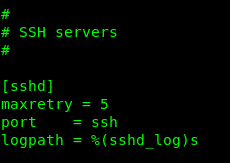
\includegraphics[scale=0.7]{fail2ban/ssh_jail}
  \caption{Configuración de jail para el servicio de ssh}
\end{figure}
\begin{figure}[H]
  \centering
  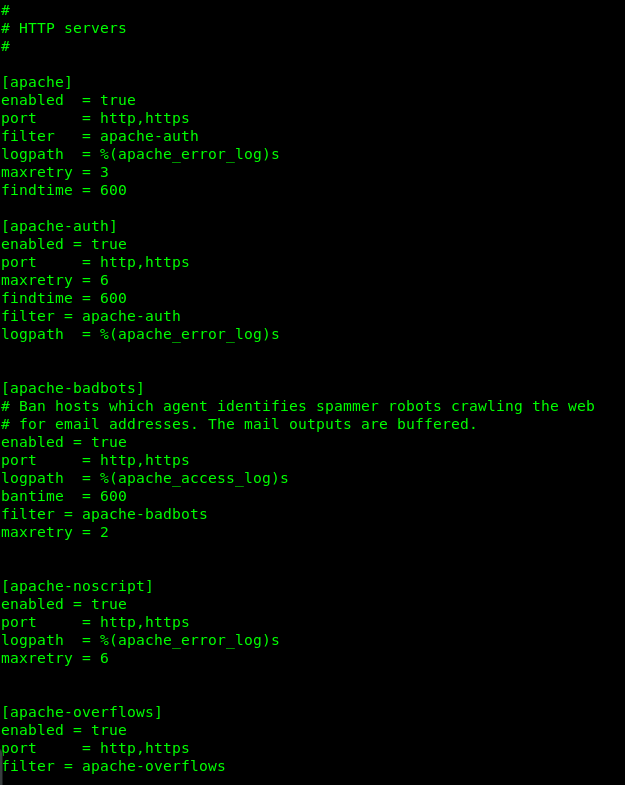
\includegraphics[scale=0.3]{fail2ban/apache_jails}
  \caption{configuración de jail para Apache}
\end{figure}

Para probar el funcionamiento de \textsf{fail2ban} se hicieron pruebas con distintas herramientas, como los \textit{benchmarks} de Apache, y verificamos el estado de las \textsf{iptables} antes y después de tales pruebas.
\begin{figure}[H]
  \centering
  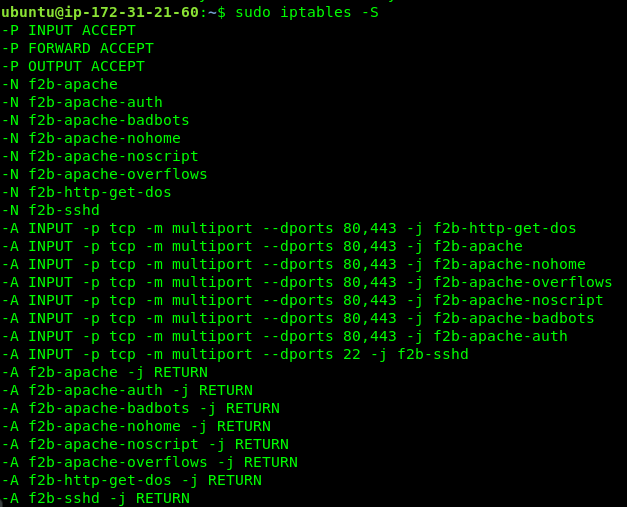
\includegraphics[scale=0.3]{fail2ban/iptables}
  \caption{estado de iptables después de configurar fail2ban}
\end{figure}
\begin{figure}[H]
  \centering
  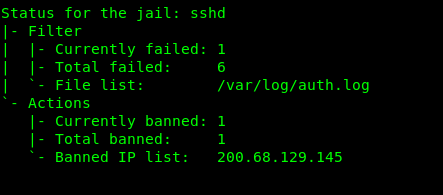
\includegraphics[scale=0.5]{fail2ban/ssh_banned_experiment}
  \caption{resultado de las pruebas para ssh}
\end{figure}
\begin{figure}[H]
  \centering
  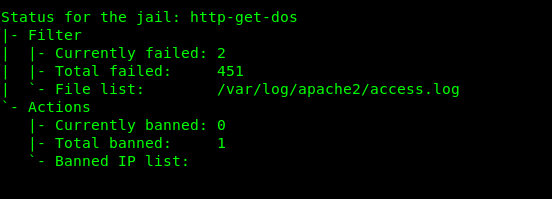
\includegraphics[scale=0.5]{fail2ban/fakeddos_test}
  \caption{resultado de una prueba de ataque DDoS}
\end{figure}
\begin{figure}[H]
  \centering
  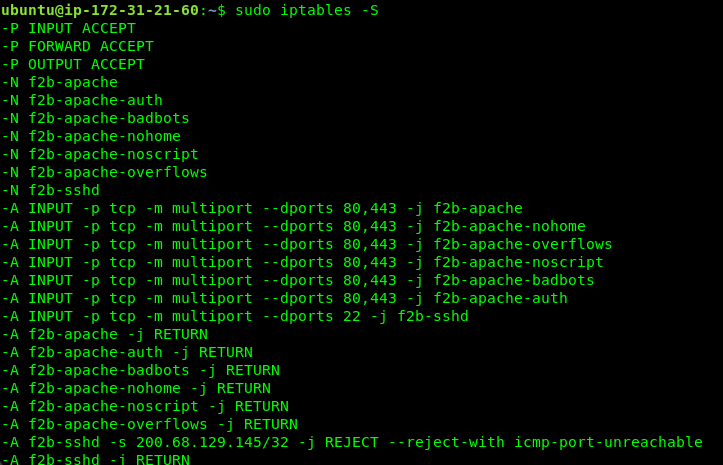
\includegraphics[scale=0.3]{fail2ban/new_iptables_with_ban}
  \caption{estado de iptables después de las pruebas}
\end{figure}

\subsection{Letsencrypt}

Se instaló el bot de \textsf{letsencrypt} en el servidor de correos y en el servidor web.

\begin{verbatim}
    $ sudo apt-get install software-properties-common
    $ sudo add-apt-repository ppa:certbot/certbot
    $ sudo apt-get update
    $ sudo apt-get install python-certbot-apache 
\end{verbatim}

Para cada servidor se corrió con \texttt{sudo certbot --apache certonly}, al terminar creó la llave y certificados. \\

Ejemplo en el servidor de correos:

\begin{center}
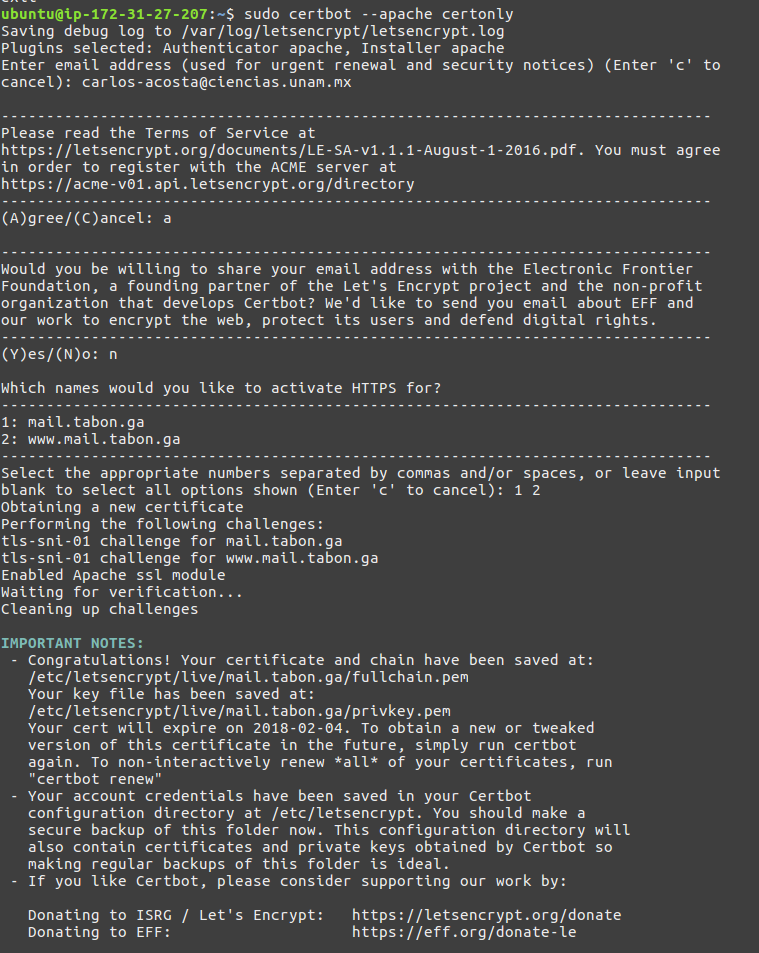
\includegraphics[scale=0.3]{mail/2}
\end{center}

\subsection{Reasignación de puerto de SSH}
A cada servidor le cambiamos el puerto del servicio \textsf{SSH} que viene por defecto (el 22) por el puerto 2200. Para realizar esto sólo bastó modificar la línea
\begin{verbatim}
Port 22
\end{verbatim}
por
\begin{verbatim}
Port 2200
\end{verbatim}
en el archivo de configuración \texttt{/etc/ssh/sshd\_config}.

\subsection{Seguridad de la base de datos}
Para garantizar que las conexiones entre cliente y servidor de la aplicación necesitamos que las conexiones con la base de datos también sean seguras. En \textsf{MySQL} están disponibles las conexiones cifradas usando el protocolo \textsf{TLS} (Transport Layer Security), el cual se asegura de que los datos que se reciban en una red pública sean confiables, además de contar con mecanismos para detectar cambios en los datos, así como pérdida o repetición de la información y validación de identidades. \\

Como primer paso, debemos asegurarnos de instalar \textsf{MySQL} de manera segura, tal como lo hicimos en la práctica 3 del curso. \\
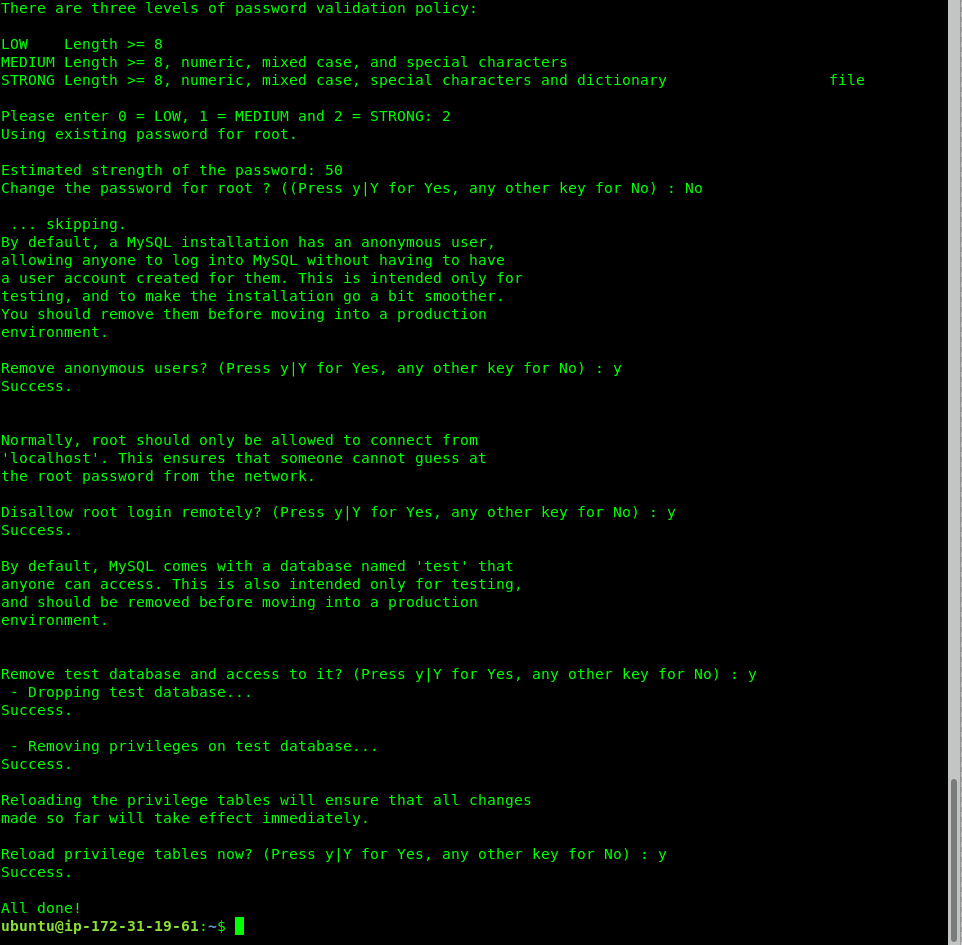
\includegraphics[width=0.7\textwidth]{mysql_secure_installation} \\
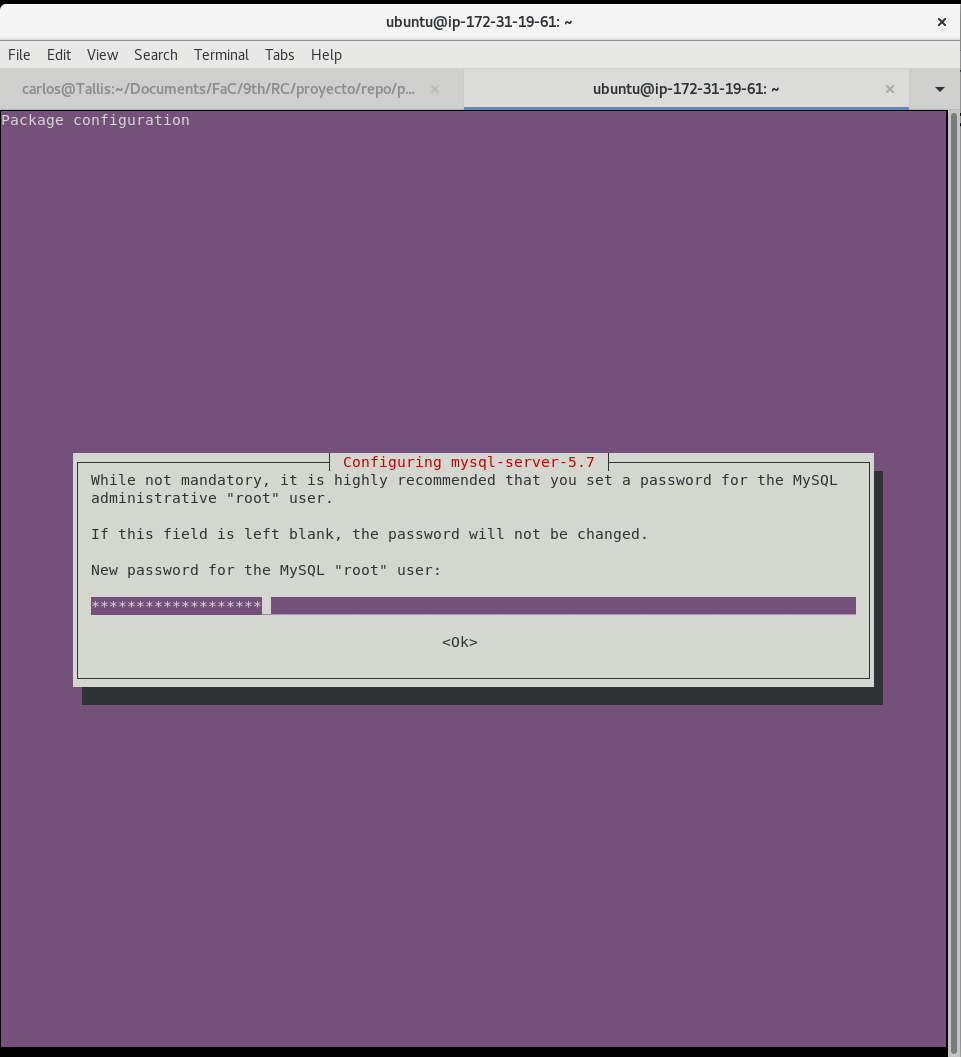
\includegraphics[width=0.7\textwidth]{mysql_install}\\


Para utilizar el cifrado de \textsf{TLS} en las conexiones de nuestra base da datos, primero hay que crear un directorio donde alojaremos las llaves y certificados requeridos para el cifrado. En este caso, elegimos tenerlas dentro del directorio de configuraciones \texttt{/etc/mysql}, pero podrían estar en cualquier otro.

\begin{verbatim}
$ cd /etc/mysql
$ sudo mkdir ssl
$ cd ssl
\end{verbatim}

Ahora creamos una llave para la \textsf{CA} (Autoridad Certificadora), de manera similar a la práctica 2 del curso,  usamos \texttt{openssl} pues ya está integrado en \textsf{Ubuntu} por defecto. \\
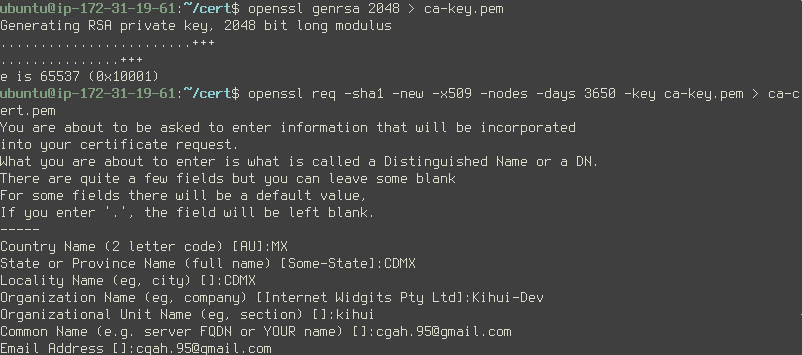
\includegraphics[width=0.8\textwidth]{mysql_cert}\\

Ahora creamos una llave para el certificado del servidor y proporcionamos la información que se nos solicite. \\
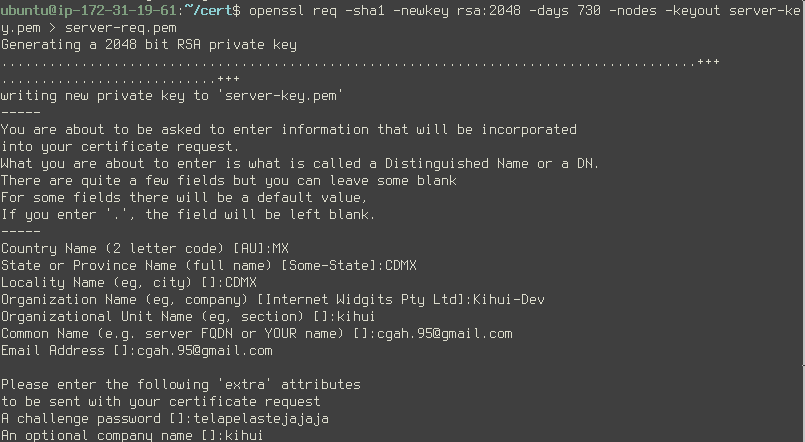
\includegraphics[width=\textwidth]{mysql_server-key}\\

Ya que tenemos tanto la llave de la \textsf{CA} como la del certificado del servidor, podemos firmar el certificado de acuerdo al formato establecido en el estándar \textbf{X.509}. \\
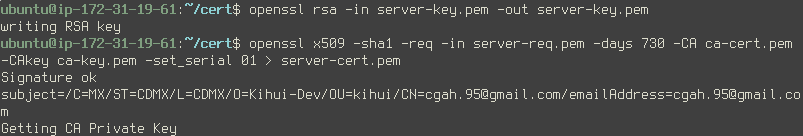
\includegraphics[width=\textwidth]{mysql_server-cert}\\

Ya que contamos con los certificados, debemos configurar \textsf{MySQL} para que cifre sus conexiones con ellos, pues si ingresamos ahora a la shell de \textsf{MySQL} y escribimos el comando \texttt{SHOW VARIABLES LIKE '\%ssl\%';} nos indicará que \textsf{SSL} no está habilitado. \\
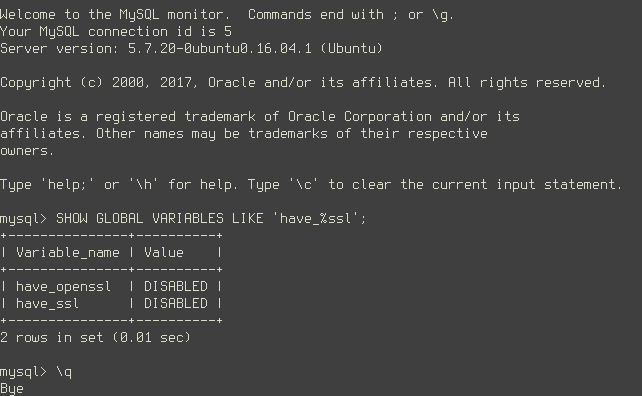
\includegraphics[width=\textwidth]{mysql_ssl-disabled} \\

Para habilitar \textsf{SSL} debemos agregar las rutas de las llaves y certificados que acabamos de crear en las variables correspondientes en el archivo de configuración de \textsf{MySQL}, que generalmente está en \texttt{/etc/mysql/my.cnf} o un archivo de nombre similar. \\
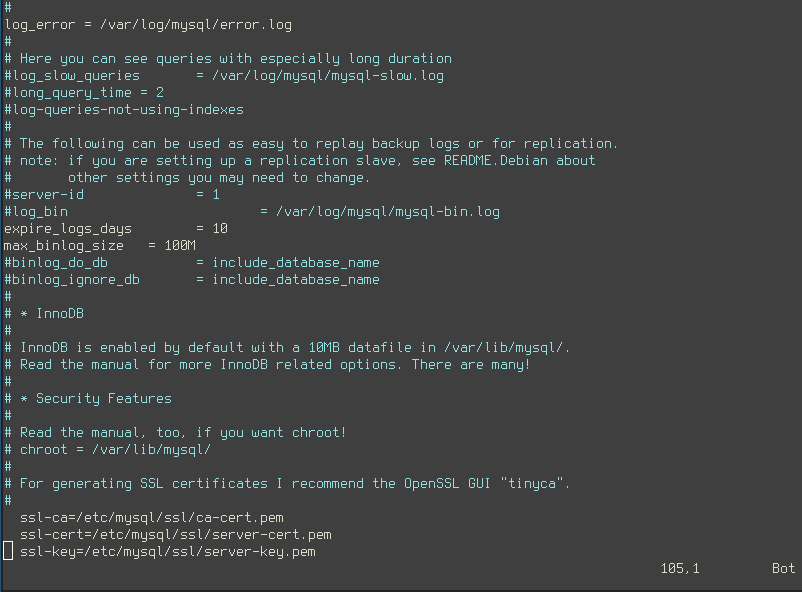
\includegraphics[width=\textwidth]{mysql_conf-ssl}\\

Si ahora ingresamos a la shell de \textsf{MySQL} y volvemos a escribir el comando \texttt{SHOW VARIABLES LIKE '\%ssl\%';} nos debe afirmar que \textsf{SSL} está habilitado, entonces las conexiones con la base de datos ya serán cifradas y tendremos mayor seguridad en la comunicación con ésta.
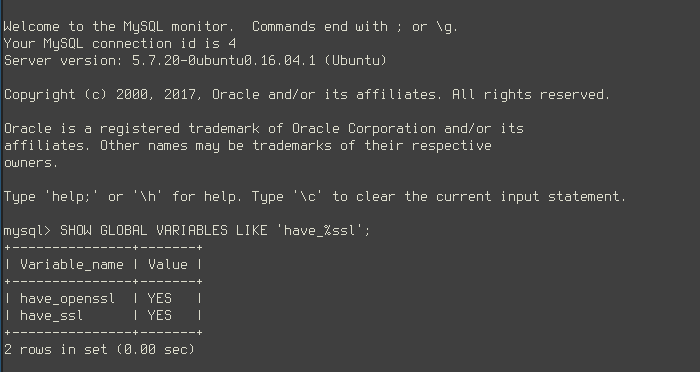
\includegraphics[width=\textwidth]{mysql_ssl-enabled}\\

\section{Servidor de correos}

Utilizamos una máquina virtual con Ubuntu 16.04. Registramos el nombre de dominio \texttt{mail.tabon.ga} para su dirección IP correspondiente, que en este caso es la \texttt{13.58.30.114}. \\
Para el funcionamiento del servidor de correos utilizamos los paquetes de \textsf{postfix}, \textsf{dovecot}, \textsf{squirrelmail} y \textsf{apache2}. Tales paquetes se instalaron de la siguiente manera: \\
\begin{verbatim}
    $ sudo apt install postfix
    $ sudo apt install dovecot-core dovecot-imapd
    $ sudo apt install apache2
\end{verbatim}

\subsection{Configuración de Postfix}
En el archivo \texttt{/etc/postfix/main.cf} se configuró lo siguiente:
\begin{verbatim}
smtpd_banner = $myhostname ESMTP $mail_name         
biff = no
append_dot_mydomain = no
readme_directory = no
smtpd_use_tls = yes
smtpd_tls_key_file = /etc/letsencrypt/live/mail.tabon.ga/privkey.pem
smtpd_tls_cert_file = /etc/letsencrypt/live/mail.tabon.ga/fullchain.pem
smtpd_tls_loglevel = 3
smtpd_tls_received_header = yes
smtpd_tls_session_cache_timeout = 3600s
tls_random_source = dev:/dev/urandom
smtpd_relay_restrictions = permit_mynetworks permit_sasl_authenticated \
                    defer_unauth_destination
myhostname = mail.tabon.ga                              
mydomain = tabon.ga
myorigin = /etc/mailname
mydestination = $myhostname, localhost.$mydomain, localhost, $mydomain
relayhost = 
mynetworks = 127.0.0.0/8, $mydomain, 132.247.0.0/16, 132.248.0.0/16
recipient_delimiter = +
inet_interfaces = all
inet_protocols = all
home_mailbox = mail/
smtpd_sasl_type = dovecot
\end{verbatim}
Se especificó donde se encuentra el certificado y llaves generados por \textsf{letsencrypt}, se modificó el banner de \textsf{smtp} y se pusieron restricciones de relay. \\
En el archivo \texttt{/etc/postfix/master.cf} se agregó lo siguiente:
\begin{verbatim}
smtp      inet  n       -       y       -       -       smtpd
submission inet n       -       y       -       -       smtpd
  -o smtpd_tls_security_level=encrypt
smtps     inet  n       -       y       -       -       smtpd
  -o smtpd_tls_wrappermode=yes
\end{verbatim}
de manera que se habilitara \textsf{smtps} y se abriera el puerto correspondiente (el 465). Finalmente se reinició el servicio con
\begin{verbatim}
    $ sudo systemctl restart postfix
\end{verbatim}

\subsection{Configuración de Dovecot}

Se modificó el archivo \texttt{/etc/dovecot/dovecot.conf} con la siguiente línea:
\begin{verbatim}
listen = *, ::
\end{verbatim}

En \texttt{/etc/dovecot/conf.d/10-auth.conf} se agregó:
\begin{verbatim}
disable_plaintext_auth = yes
auth_mechanisms = plain login
\end{verbatim}

En \texttt{/etc/dovecot/conf.d/10-mail.conf}:
\begin{verbatim}
mail_location = maildir:~/mail
\end{verbatim}

Y en \texttt{/etc/dovecot/conf.d/10-ssl.conf}
\begin{verbatim}
ssl = yes
ssl_cert = </etc/letsencrypt/live/mail.tabon.ga/fullchain.pem
ssl_key = </etc/letsencrypt/live/mail.tabon.ga/privkey.pem
\end{verbatim}

\subsection{Configuración de Squirrelmail}
Se corrió el bot de configuración de Squirrelmail:
\begin{verbatim}
    $ sudo squirrelmail-configure
\end{verbatim}

Por lo que se mostró el menú de configuración:

\begin{verbatim}
SquirrelMail Configuration : Read: config.php (1.4.0)
---------------------------------------------------------
Main Menu --
1.  Organization Preferences
2.  Server Settings
3.  Folder Defaults
4.  General Options
5.  Themes
6.  Address Books
7.  Message of the Day (MOTD)
8.  Plugins
9.  Database
10. Languages

D.  Set pre-defined settings for specific IMAP servers

C   Turn color on
S   Save data
Q   Quit

Command >> 
\end{verbatim}

Se seleccionó la opción 2. Se procedió a configurar las opciones de SMTP e IMAP, que quedaron de ka siguiente manera:

\begin{verbatim}
SquirrelMail Configuration : Read: config.php (1.4.0)
---------------------------------------------------------
Server Settings

General
-------
1.  Domain                 : tabon.ga
2.  Invert Time            : false
3.  Sendmail or SMTP       : SMTP

IMAP Settings
--------------
4.  IMAP Server            : mail.tabon.ga
5.  IMAP Port              : 993
6.  Authentication type    : login
7.  Secure IMAP (TLS)      : true
8.  Server software        : dovecot
9.  Delimiter              : /

SMTP Settings
-------------
4.   SMTP Server           : mail.tabon.ga
5.   SMTP Port             : 465
6.   POP before SMTP       : false
7.   SMTP Authentication   : none
8.   Secure SMTP (TLS)     : true
9.   Header encryption key : 
\end{verbatim}

% | egrep -v "(.*#.*|^$)"

\subsection{Configuración de Apache}

Se habilitaron los modulos necesarios para que \textsf{https} funcione \\
\begin{verbatim}
    $ sudo a2enmod ssl
    $ sudo a2enmod headers
    $ sudo a2enmod rewrite
\end{verbatim}

Se copió el archivo de squirrelmail de apache a los sitios disponibles de apache, se habilitó junto con \textsf{default-ssl} y se deshabilitó el sitio por defecto de Apache. \\
\begin{verbatim}
    $ sudo cp /etc/squirrelmail/apache.conf \
        /etc/apache2/sites-available/squirrelmail.conf
    $ sudo a2ensite squirrelmail.conf
    $ sudo a2ensite default-ssl
    $ sudo a2dissite 000-default.conf
\end{verbatim}

En el archivo \texttt{/etc/apache2/conf-enabled/security.conf} se modificó la firma de Apache para que no muestre su versión y el sistema operativo en uso. \\
\begin{verbatim}
ServerTokens Prod
ServerSignature Off
\end{verbatim}

El archivo \texttt{/etc/apache2/sites-available/squirrelmail.conf} quedó de la siguiente manera
\begin{verbatim}
Alias /mail /usr/share/squirrelmail
<Directory /usr/share/squirrelmail>
  Options FollowSymLinks
  <IfModule mod_php.c>
    php_flag register_globals off
  </IfModule>
  <IfModule mod_dir.c>
    DirectoryIndex index.php
  </IfModule>
  <Files configtest.php>
    order deny,allow
    deny from all
    allow from 127.0.0.1
  </Files>
</Directory>

RedirectMatch ^/$ /mail/
<IfModule mod_rewrite.c>
  <IfModule mod_ssl.c>
    <Location /squirrelmail>
      RewriteEngine on
      RewriteCond %{HTTPS} !^on$ [NC]
      RewriteRule . https://%{HTTP_HOST}%{REQUEST_URI}  [L]
    </Location>
  </IfModule>
</IfModule>
\end{verbatim}

El archivo \texttt{/etc/apache2/sites-available/default-ssl.conf} quedó de la siguiente manera:
\begin{verbatim}
<IfModule mod_ssl.c>
    <VirtualHost _default_:443>
        ErrorLog ${APACHE_LOG_DIR}/error.log
        CustomLog ${APACHE_LOG_DIR}/access.log combined
        SSLEngine on
        SSLCertificateFile    \
            /etc/letsencrypt/live/mail.tabon.ga/fullchain.pem
        SSLCertificateKeyFile \
            /etc/letsencrypt/live/mail.tabon.ga/privkey.pem
        <FilesMatch "\.(cgi|shtml|phtml|php)$">
            SSLOptions +StdEnvVars
        </FilesMatch>
        <Directory /usr/lib/cgi-bin>
            SSLOptions +StdEnvVars
        </Directory>
        ServerName mail.tabon.ga
        ServerAlias www.mail.tabon.ga
        Header always set Strict-Transport-Security \
            "max-age=31536000; includeSubDomains; preload"
 
    </VirtualHost>
</IfModule>
\end{verbatim}

Al finalizar estas configuraciones se reiniciaron los servicios con \textsf{systemctl}. \\

Pudimos ver entonces la página de inicio de Squirrelmail al ingresar a \texttt{mail.tabon.ga}: \\
\begin{center}
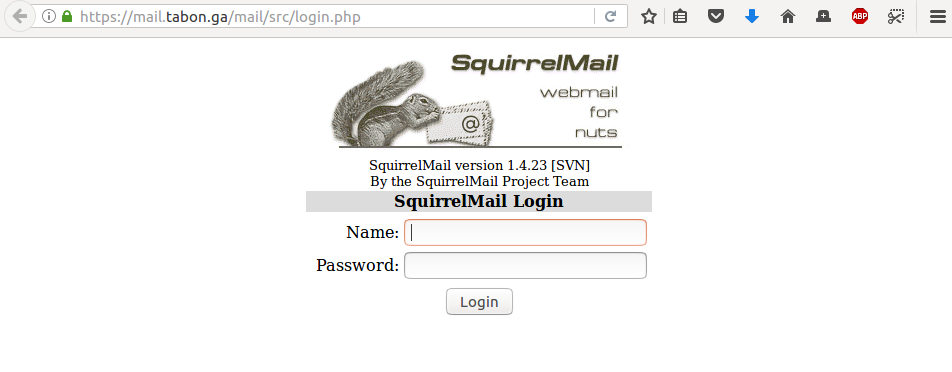
\includegraphics[scale=0.4]{mail/04} \\
\end{center}

Se agregaron los registros DNS de tipo MX y SPF para el dominio \texttt{tabon.ga} que son necesarios para el correcto funcionamiento del sistema, de manera que se acepte el correo que se manda al servidor asociado a tal dominio y se mande al servidor de correos, y que se evite que los correos mandados desde éste se vayan a spam. \\

\begin{center}
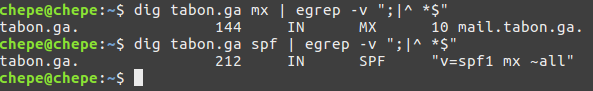
\includegraphics[scale=0.5]{mail/01} \\
\end{center}

\subsection{Reglas de firewall}
\begin{center}
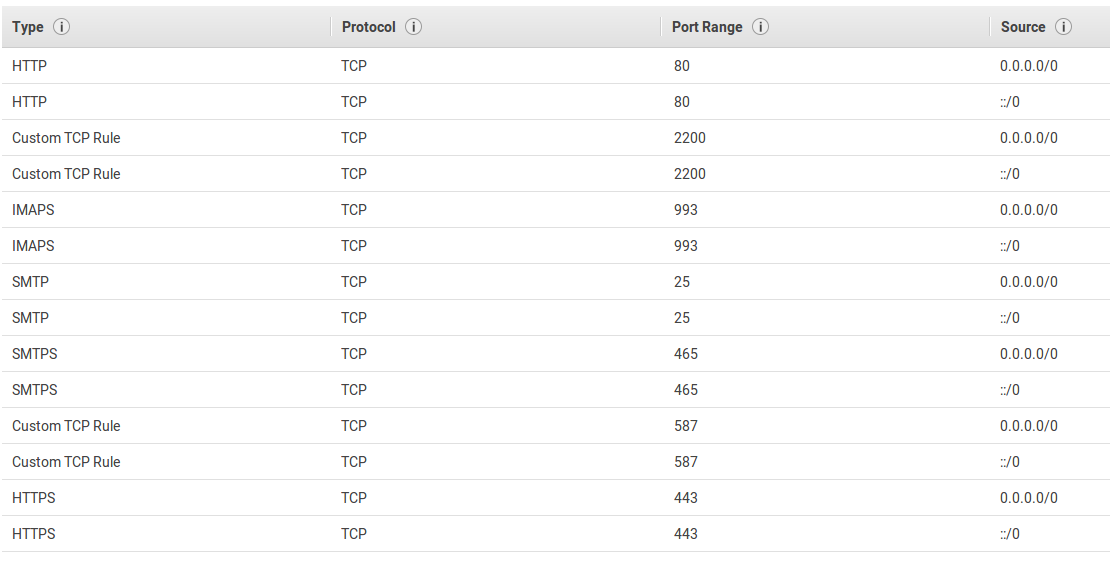
\includegraphics[scale=0.3]{mail/03} \\
\end{center}

\newpage

\subsection*{Comentarios sobre el desarrollo del proyecto}
% We didn't deserve this
Intentamos hacer una aplicación lo más sencilla posible, minimizando la carga de trabajo que podría tener el servidor de aplicación, para enforcarnos en los aspectos más importantes que requería el proyecto: la comunicación entre los servidores y la seguridad en esta comunicación. %pero todo cambió cuando la nación del fuego atacó.

\end{document}
